\documentclass{article}

% \usepackage{standalone}
 \usepackage{graphicx}
% \usepackage{media9}
%\graphicspath{{./images/}}
% \usepackage{amsmath}
\usepackage{multicol}
\usepackage{hyperref}
% \usepackage{setspace}                       \usepackage{geometry}          
%  \usepackage{longtable}                      
% \usepackage{chicago}                  
% \usepackage{times} 
% \usepackage{paracol}   % parallel columns    
% \usepackage[dvipsnames]{xcolor}       \usepackage{calc}                                      

% \usepackage{tikz}
% \usetikzlibrary{positioning, shadows, arrows, automata, shapes, calc, decorations.pathreplacing,calligraphy}

\title{Notes on Experiments}
\author{KLMW}
\begin{document}
\maketitle
\tableofcontents \newpage
\section{Notes on Experiments}
This is a record of experiments testing the effect of  varying parameters. The tests are grouped in two parts: tests of the base model of city and the production sector, and tests of the housing market parameters. 

In the first part the goal is to ensure that the platform underlying the housing market behaves as expected. One important policy result was found: Transportation costs, which are under the control of local governments, have a very large effect.

In the second part we find that the proportion of owner occupiers is sensitive to  several policy instruments. 

Complex combinations of policies are computationally  intensive and are not explored in this section.

\vspace{.5cm}

{\tiny
BASELINE PARAMETERS
\begin{verbatim}

        # LABOUR MARKET AND FIRM PARAMETERS
            'subsistence_wage': 40000., # psi
            'init_city_extent': 10.,    # CUT OR CHANGE?
            'seed_population': 400,
            'init_wage_premium_ratio': 0.2, # 1.2, ###

            # PARAMETERS MOST LIKELY TO AFFECT SCALE
            'c': 300                             ### .0,                            ###
            'price_of_output': 10,                 ######
            'density':600,                         #####
            'A': 3000,
            'alpha': 0.18,
            'beta':  0.75,
            'gamma': 0.12, ### reduced from .14
            'overhead': 1.5,
            'mult': 1.2,
            'adjN': 0.15,
            'adjk': 0.10,
            'adjn': 0.15,
            'adjF': 0.02,
            'adjw': 0.05, 
            'dist': 1, 
            'init_F': 100.0,
            'init_k': 500.0,
            'init_n': 100.0,

            # HOUSING AND MORTGAGE MARKET PARAMETERS
            'mortgage_period': 5.0,       # T, in years
            'working_periods': 40,        # in years
            'savings_rate': 0.3,
            'discount_rate': 0.07,        # 1/delta    Check THIS
            'r_prime': 0.05,
            'r_margin': 0.01,
            'property_tax_rate': 0.04,     # tau, annual rate, was c
            'housing_services_share': 0.3, # a
            'maintenance_share': 0.2,      # b
            'max_mortgage_share': 0.9,
            'ability_to_carry_mortgage': 0.28,
            'wealth_sensitivity': 0.1,
            'capital_gains_tax_person':   0.0, # share 0-1
            'capital_gains_tax_investor': 1, # share 0-1
    
\end{verbatim}
}
\newpage

% \subsection{parameters}
% \begin{verbatim}

% \end{verbatim}
\section{Base model of city and the production sector}
 \subsection{Change Density}
 This experiment verifies that the labour-market/urban model that is the platform for the housing market analysis behaves exactly as expected when density changes. mpl, n, N, F, E, and k all rise. %Population rises with 

 The fraction owner-occupiers falls earlier with increasing density due to more rapid financialization and the potential rent capture increases, and  not to changing housing form. It seems later entrants do not purchase. The transition is achieved in about two full generations  in our model. The timing will be sensitive to the specific parameterization.
 

 \hspace*{-2cm}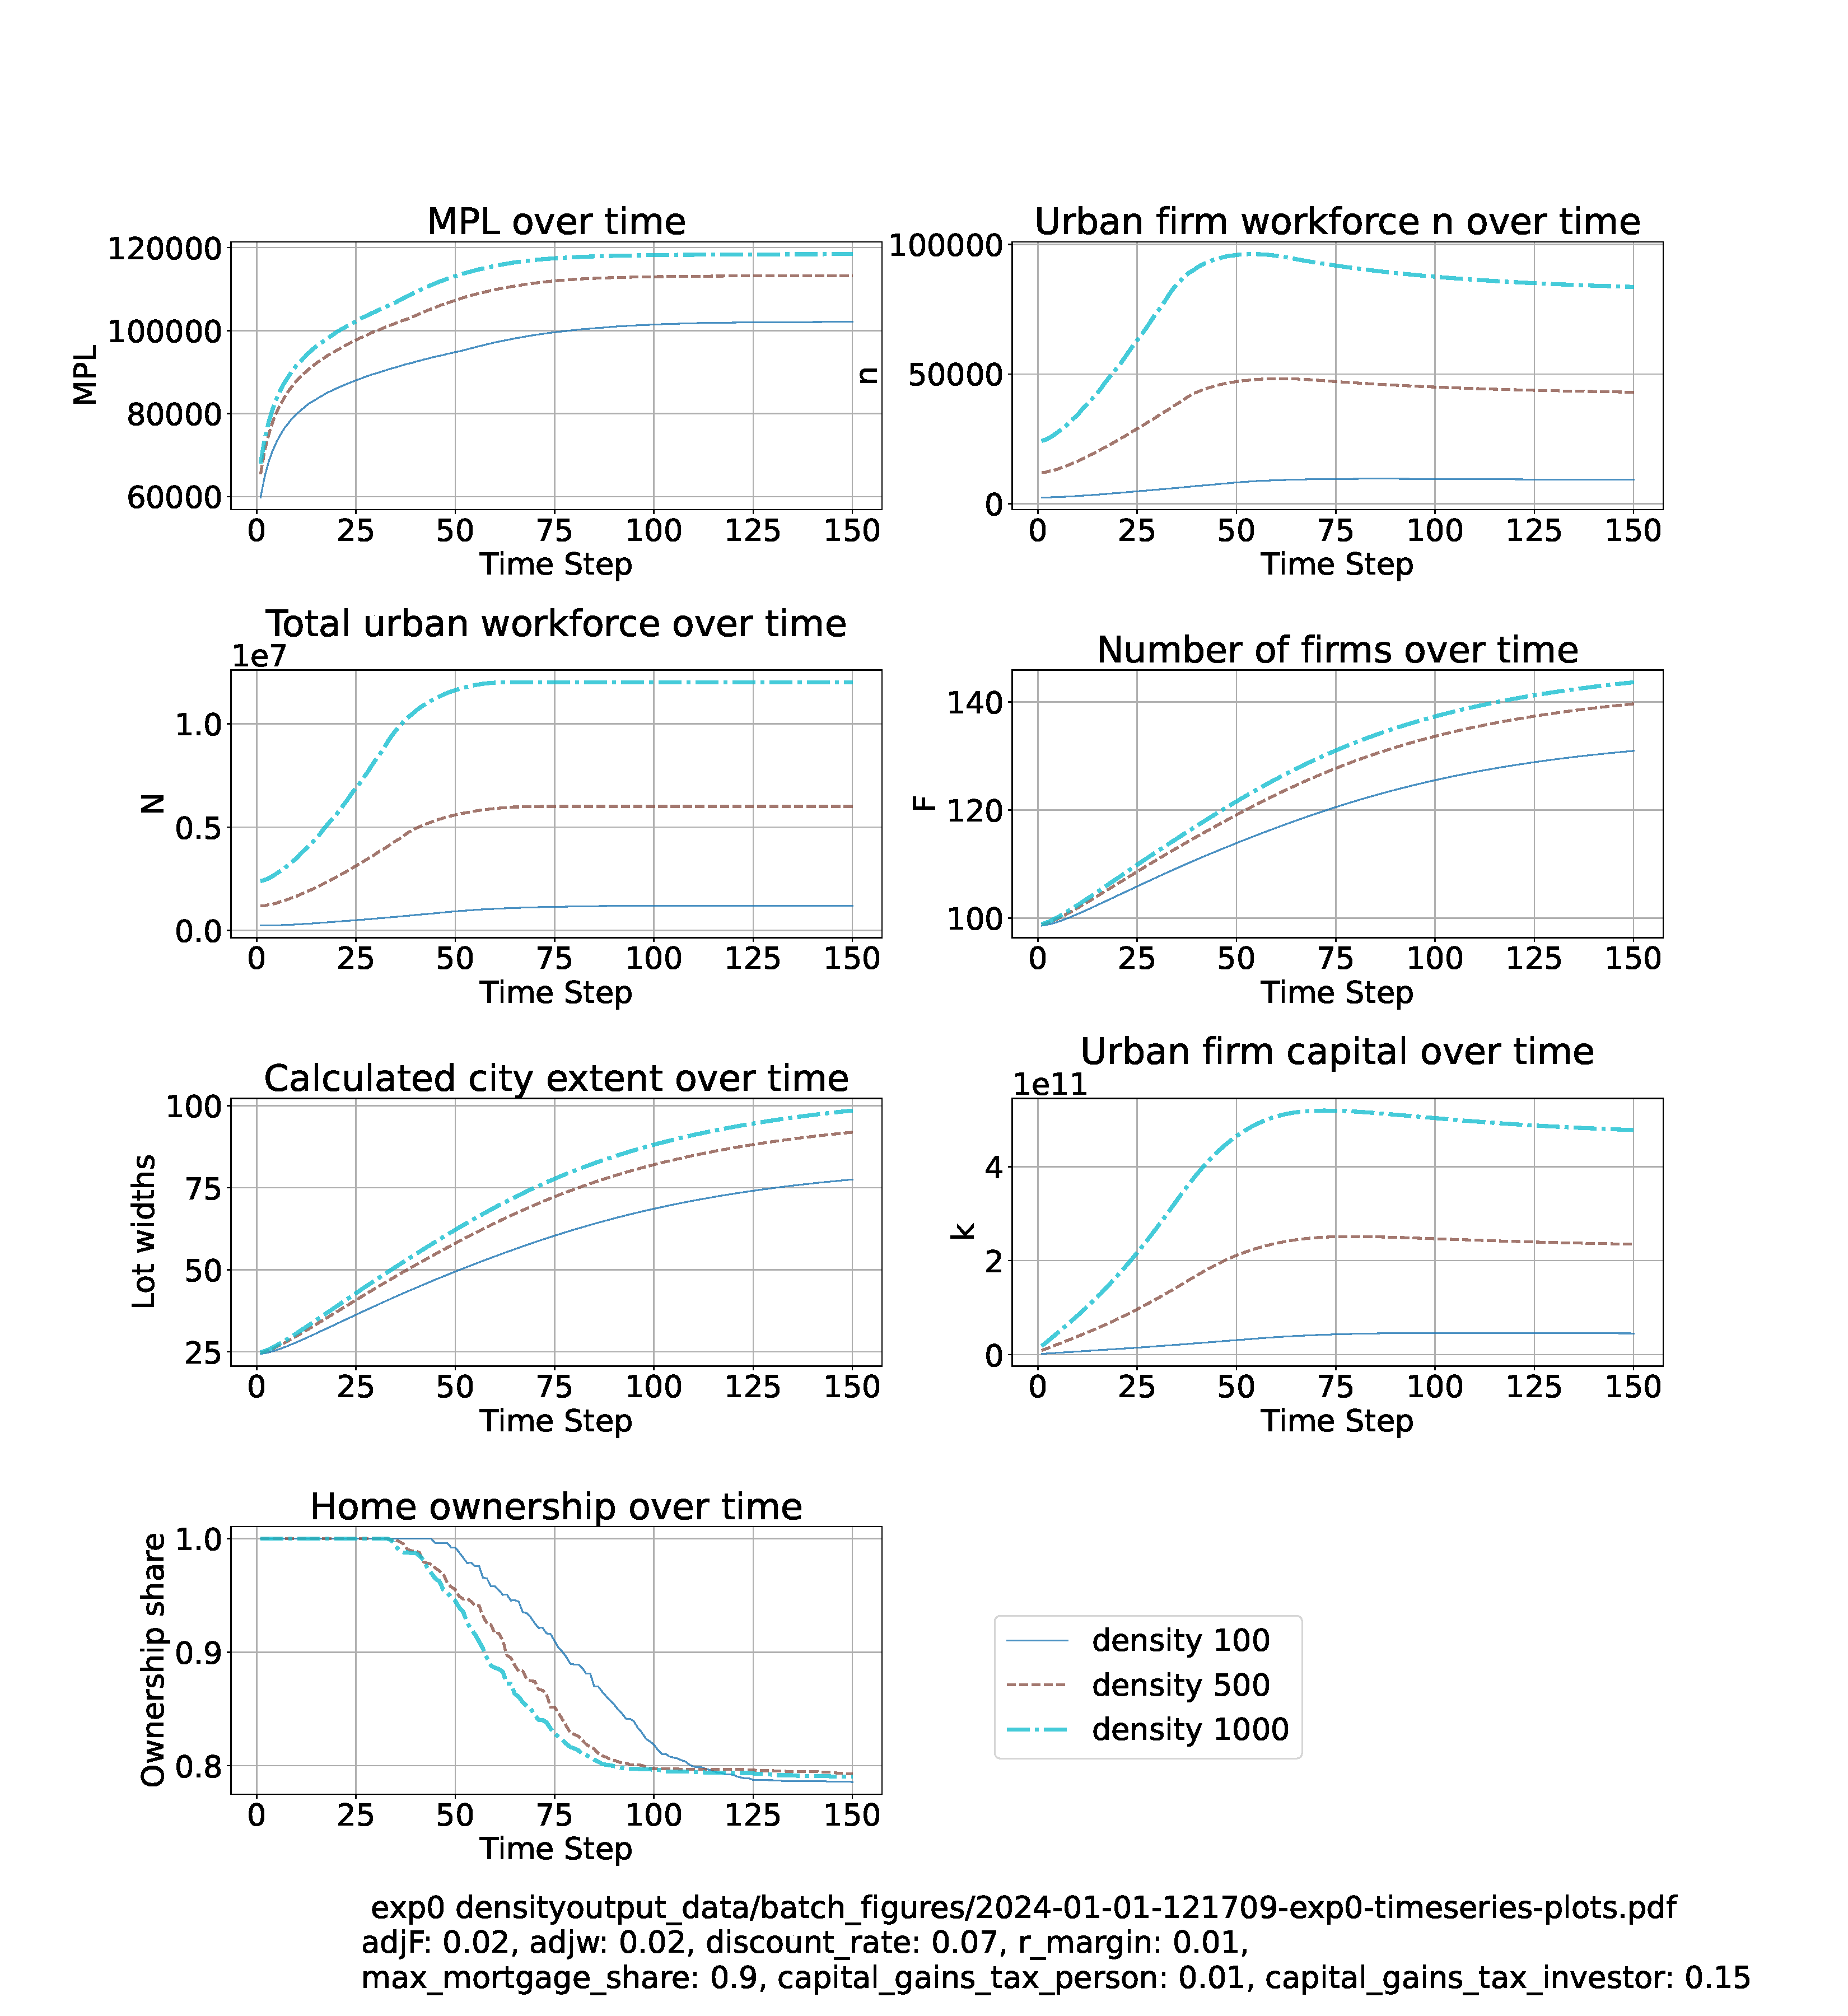
\includegraphics[trim= 1.5cm 3.65cm 2cm 4.0cm, clip, scale=.3]{Density-3-150.pdf}

\newpage %%%%%%%%%%%%%%%%%%%%%%%%%%%%%%%%%%

\subsection{High Gamma}
Very high levels of the agglomeration parameter Gamma are implausible. They drive up marginal productivity, causing very rapid growth, drive down firm size because the first worker is extremely productive but the MPL falls rapidly. Very small firms with high levels of capital multiply. Rapidly rising prices encourage investors while savings-limited owner-occupiers are squeezed out.

Higher agglomeration effects  make land rents higher and increase the gains to investors, resulting in more rapid financialization of the housing stock.

%   we can check
 
% \begin{tabular}{|c|c||c|c||c|c|}
% mpl  & up   & n   & up & N   &  up \\
% F    & up   & E   &  up  &  k & up
% \end{tabular} 

 \hspace*{-2.5cm}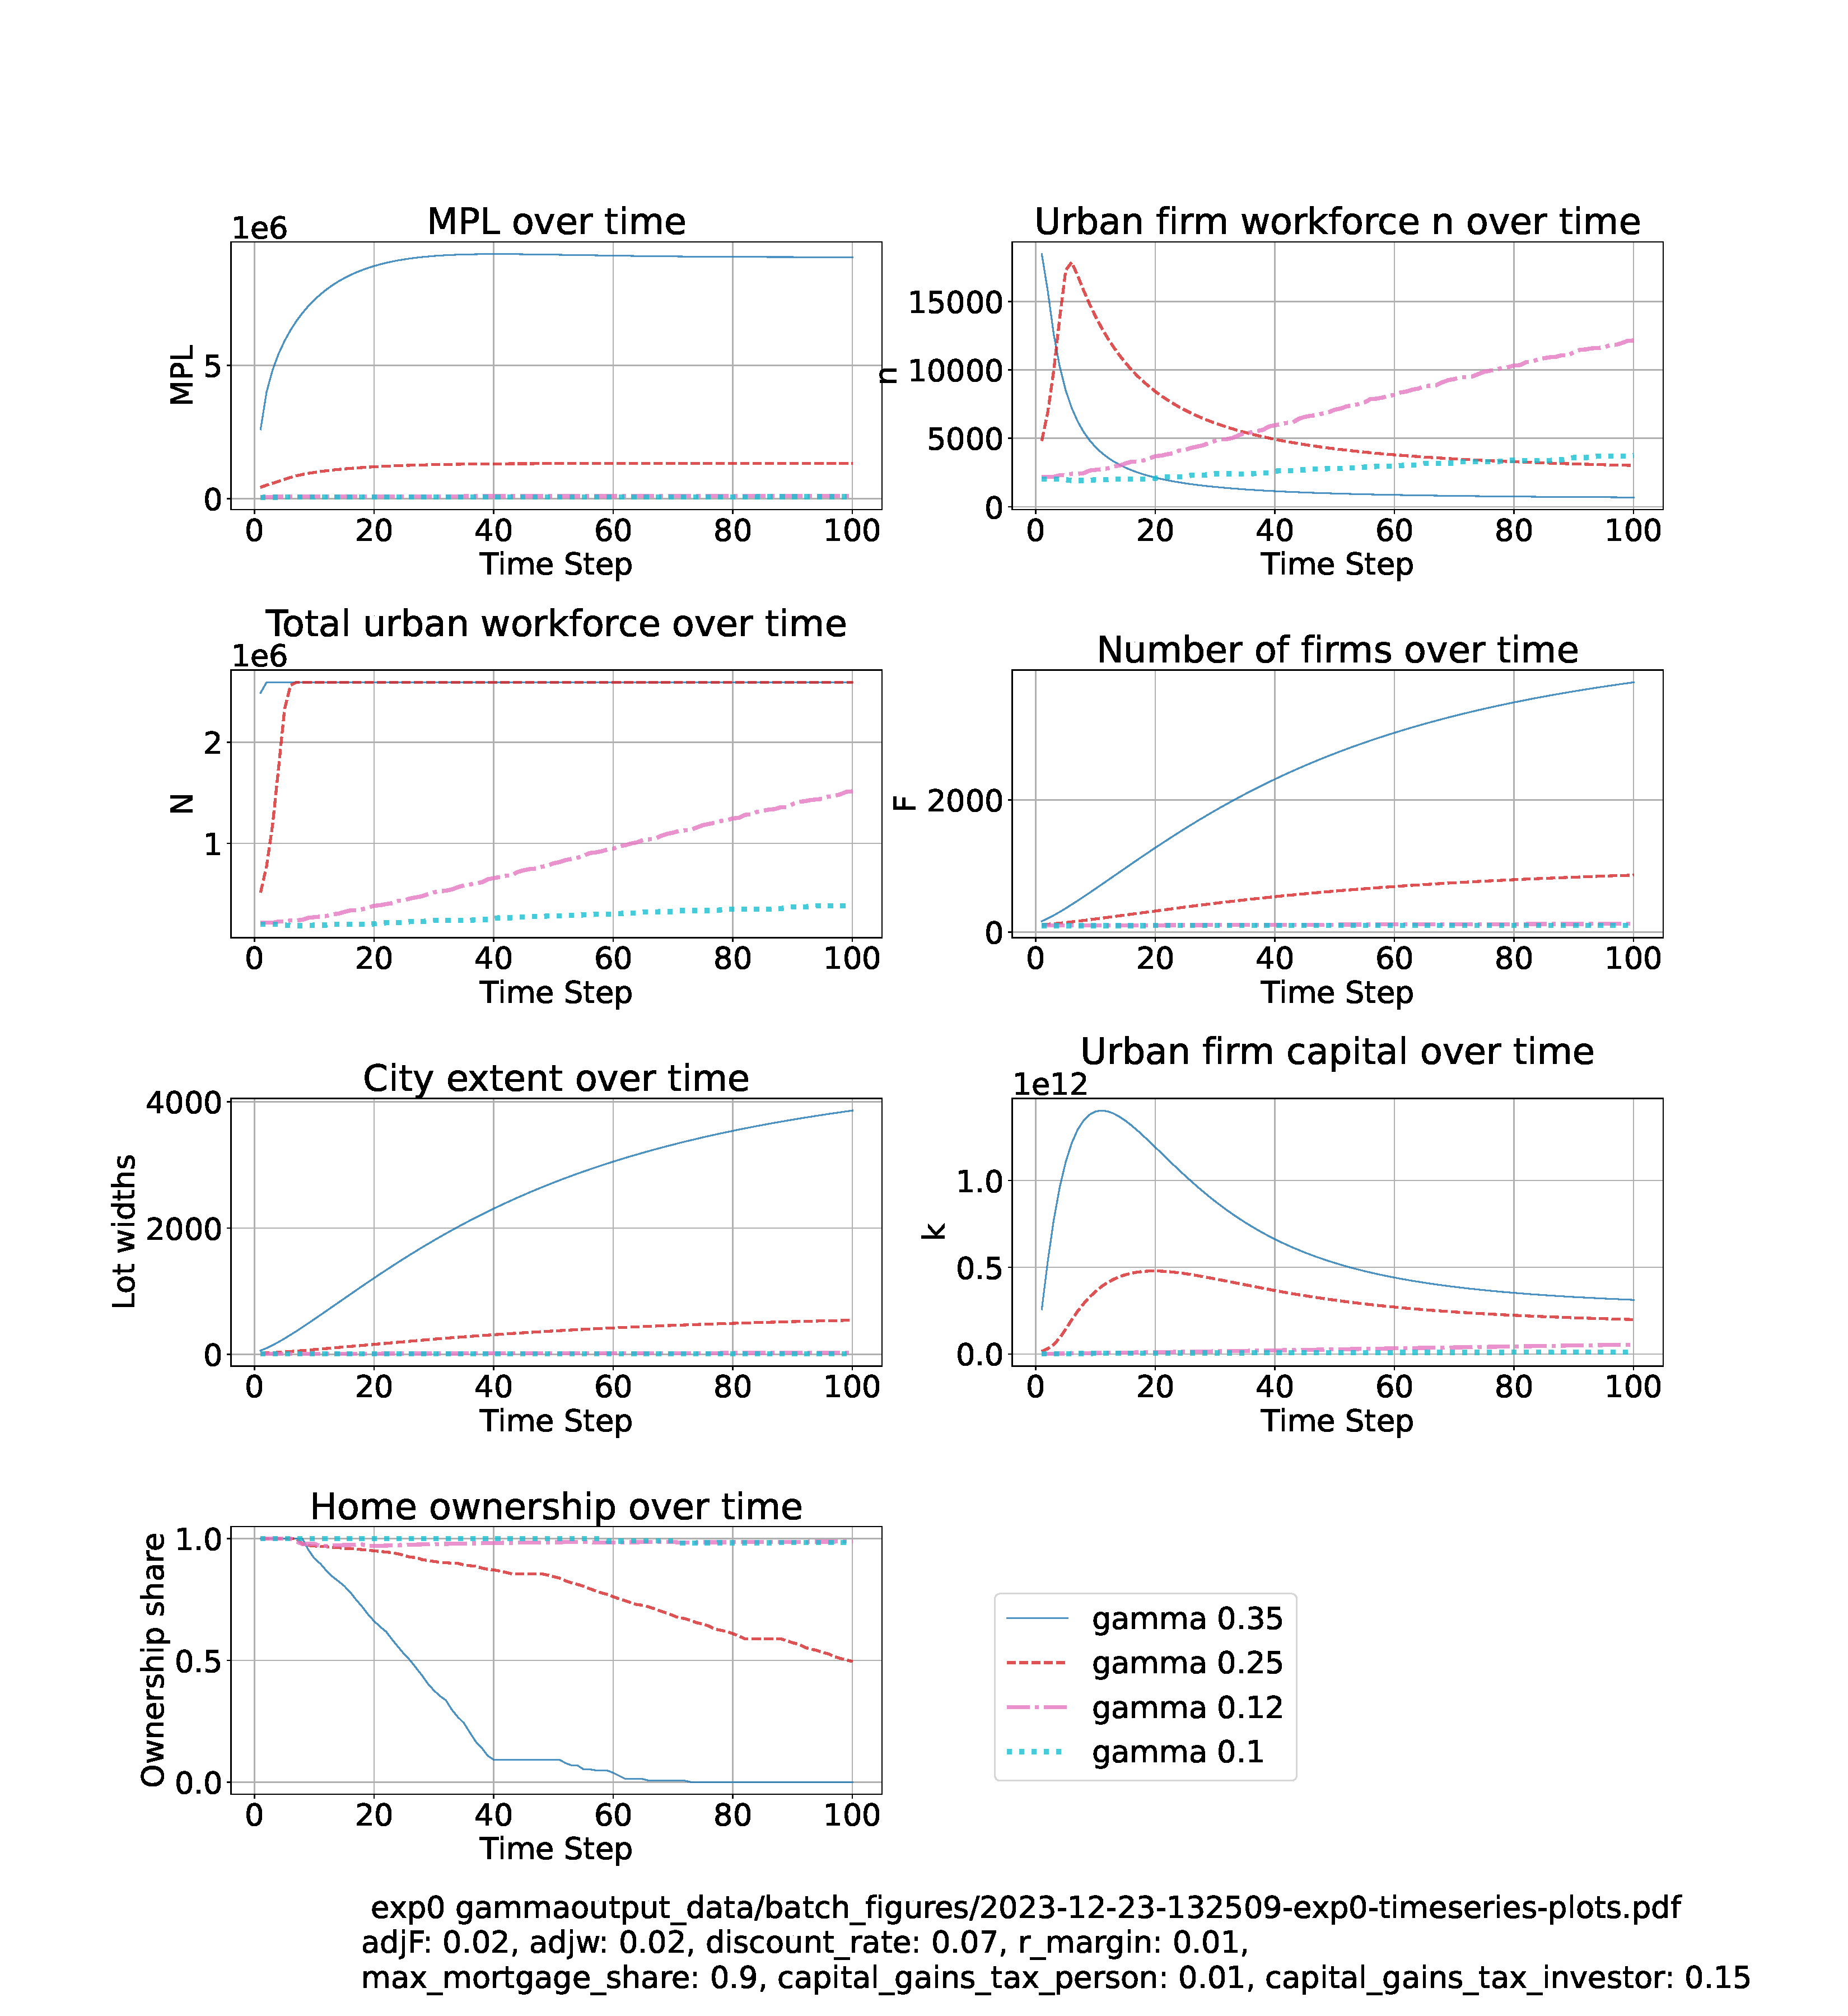
\includegraphics[trim= 1.5cm 3.65cm 2cm 4.0cm, clip, scale=.28]{fig/Analysis/Gamma-5-30.pdf}

\newpage %%%%%%%%%%%%%%%%%%%%%%%%%%%%%%%%%%

\subsection{Low Gamma}
Low levels of the agglomeration parameter Gamma are plausible but city growth requires a level high enough to overcome decreasing returns in production.

At near-zero levels population is hiring at the firm level sharply affects  the marginal product and randomization in saving the share of housing that is owner occupied.
 
% \begin{tabular}{|c|c||c|c||c|c|}
% mpl  & up   & n   & up & N   &  up \\
% F    & up   & E   &  up  &  k & up
% \end{tabular} 

 \hspace*{-2.5cm}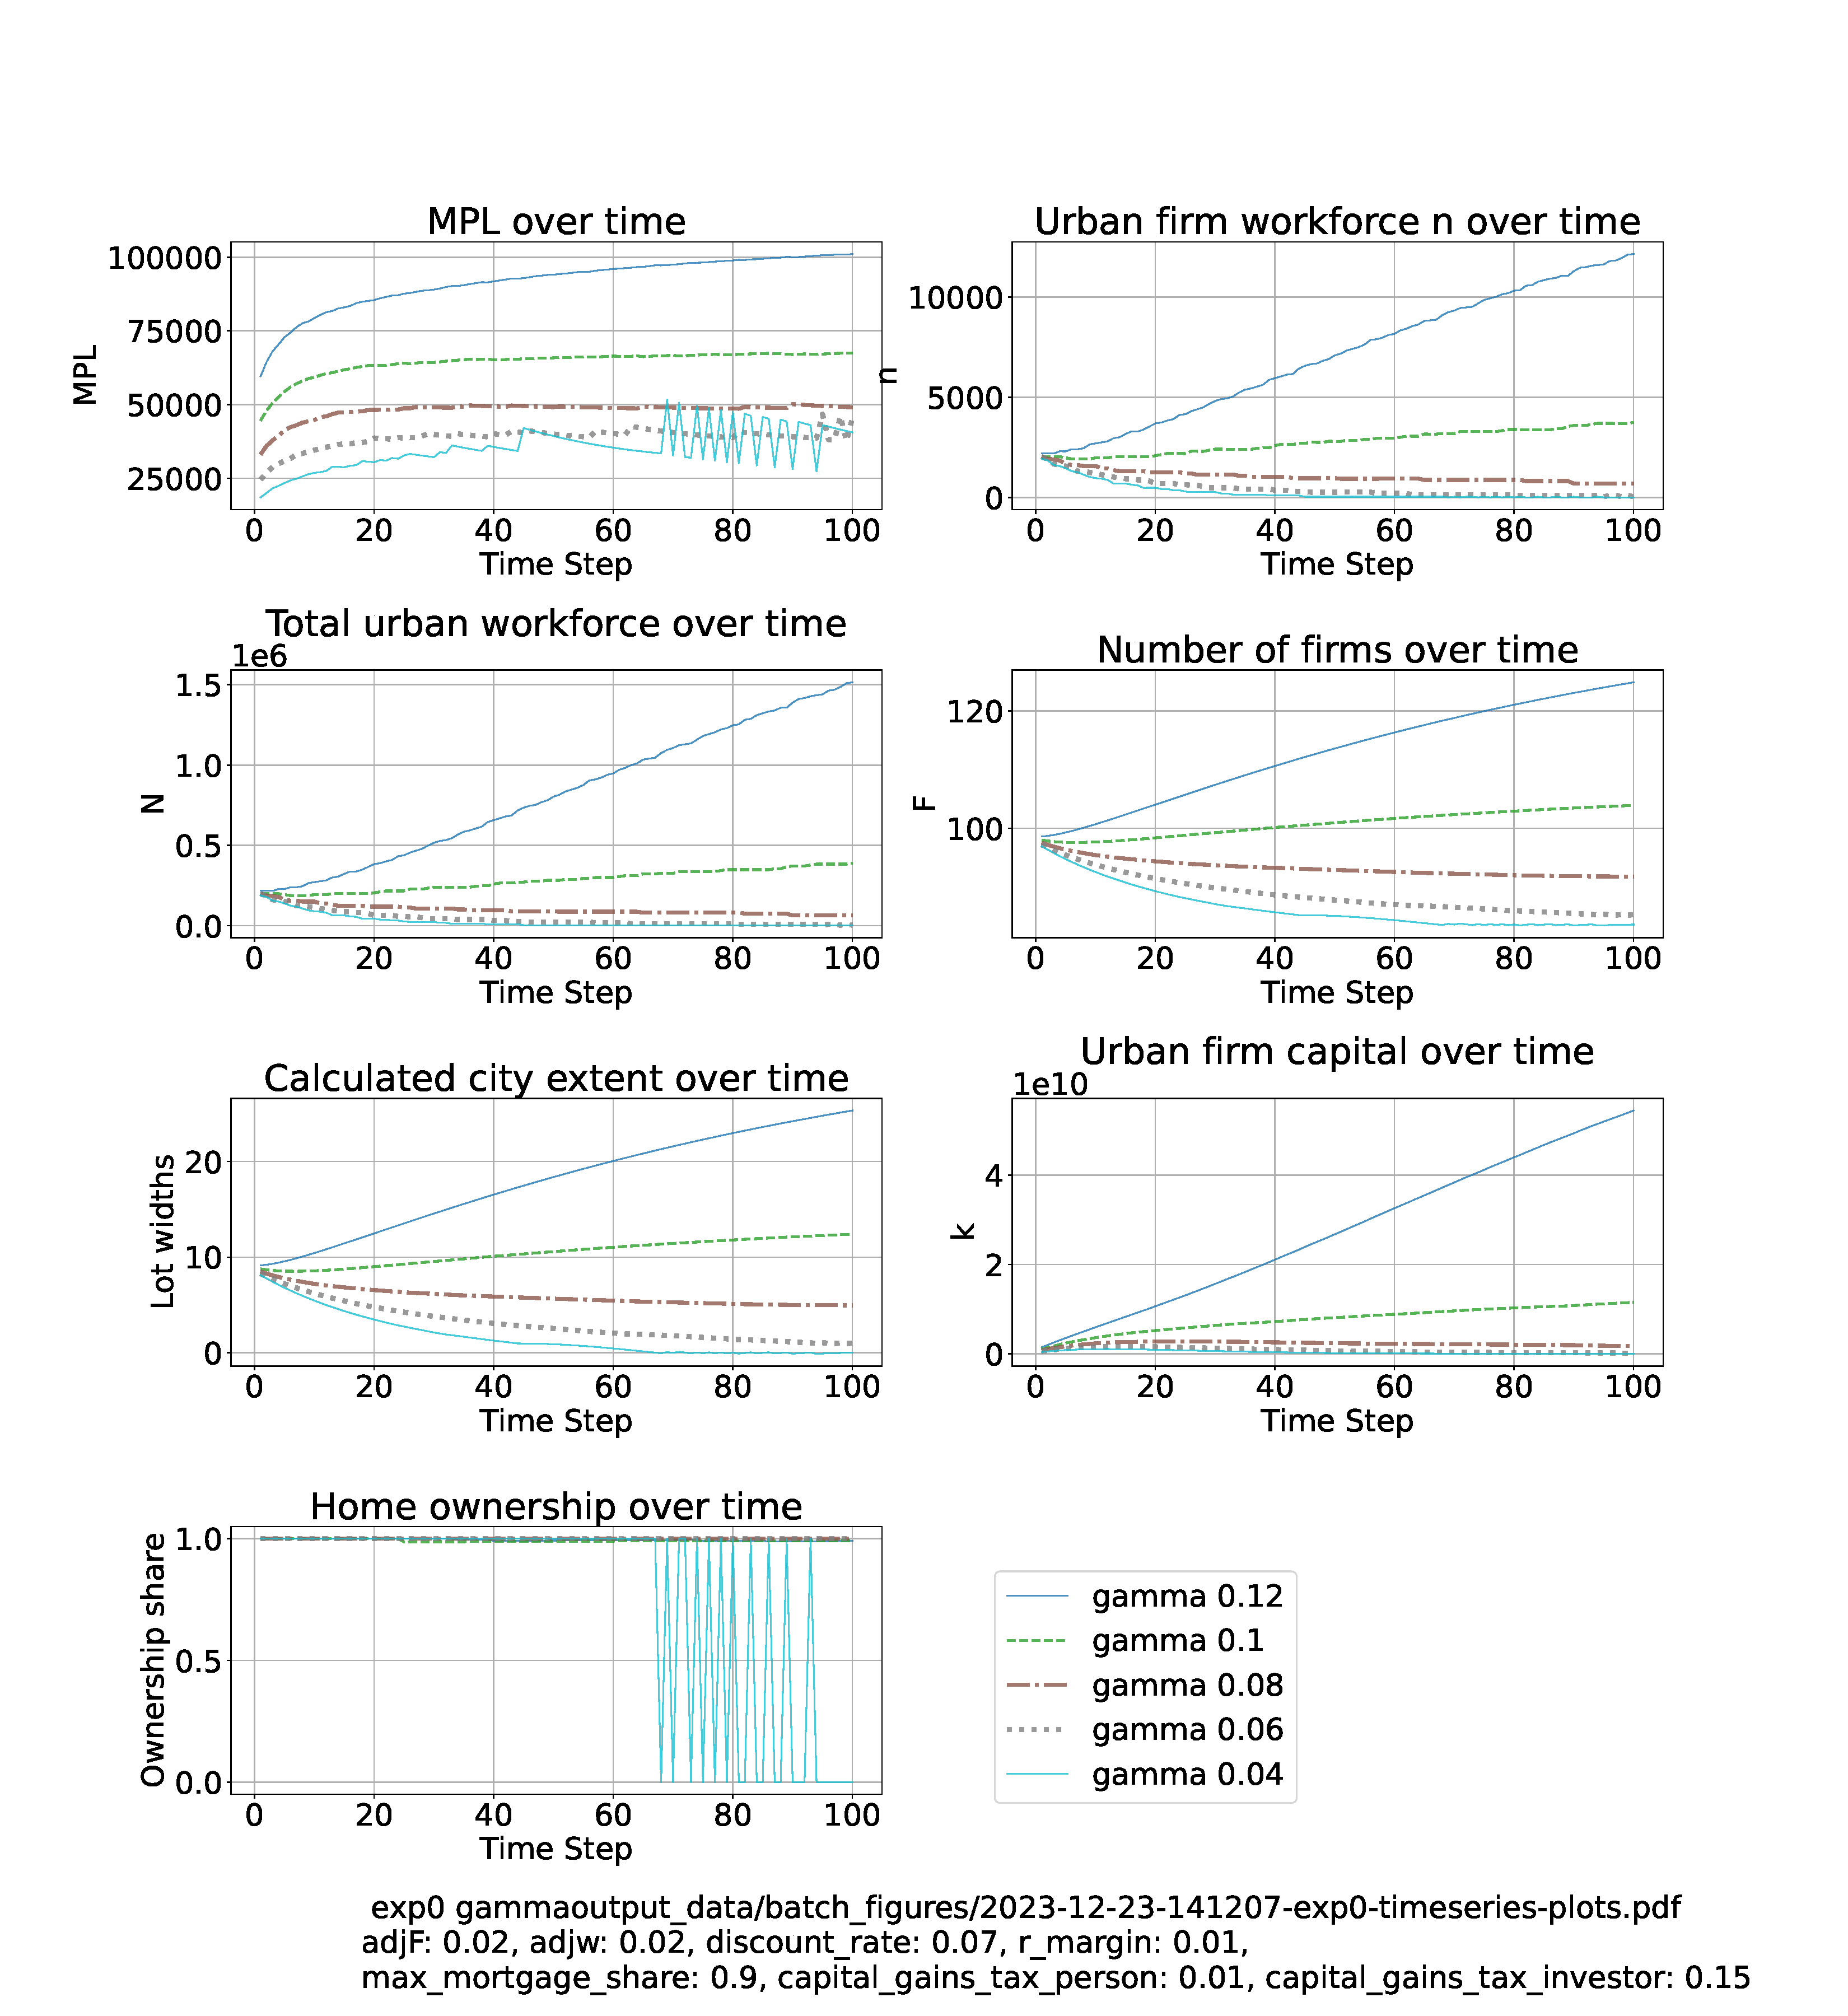
\includegraphics[trim= 1.5cm 3.65cm 2cm 4.0cm, clip, scale=.3]{fig/Analysis/Gamma-low-5-30.pdf}

\newpage %%%%%%%%%%%%%%%%%%%%%%%%%%%%%%%%%%

\subsection{Change adjF - the growth rate of number of firms }

\begin{multicols}{2}
\begin{tabular}{c|c}
  mpl   &  up\\
  n   &  dn\\
  N   &  up\\
  F   & up \\
  E   &  up\\
  k   & dn
\end{tabular}

  notice the way firm number and size reverse as the adjustment speed changes. This makes sense
  
\end{multicols}

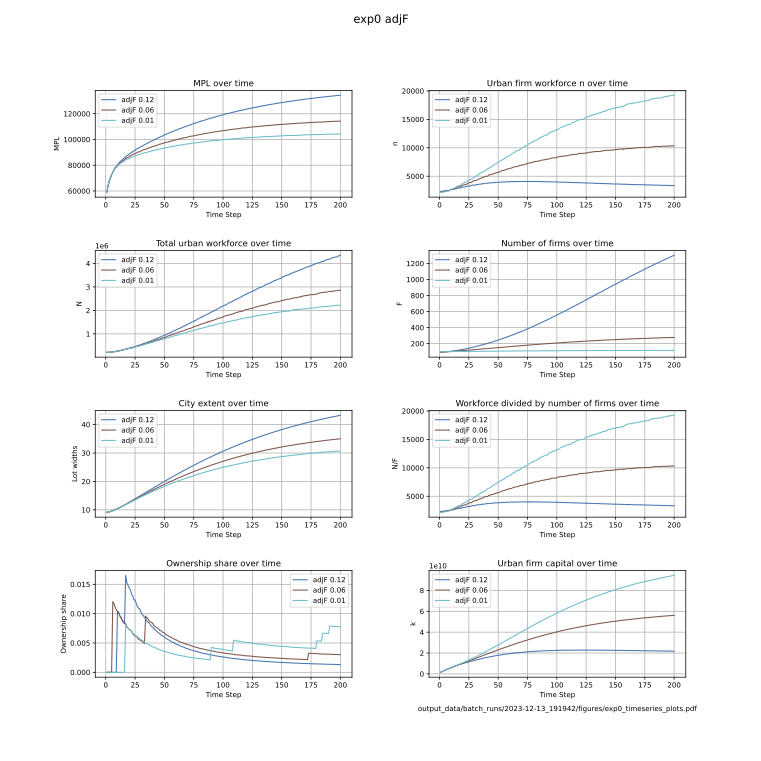
\includegraphics[scale=.55]{fig/Analysis/AdjF.png}

Notice too how MPL  is higher with a more rapid firm size adjustment. It keeps  firm workforce size down and pushes up MPL down, 

  Interestingly, city size is larger with faster growth of firm numbers. this is likely because with more firms hiring the population of the city grows faster.

  Ownership bounces around due to randomization of savings.


TO DO RE RUN WITH CURRENT PARAMETSRS AND GRAPHING
%%%%%%%%%%%%%%%%%%%%%%%%%%%%%%%%%%%%%%%%%%%%%
\newpage
% \subsection{parameters}
% \begin{verbatim}

% \end{verbatim}

 \subsection{x12-15 010050, Change  Both adjF and adjn}

 REDO AS 2x2
\begin{multicols}{2}
\begin{tabular}{c|c}
  mpl  &  \\
  n   &  \\
  N   &  \\
  F   &  \\
  E   &  \\
  k   & 
\end{tabular} 
Only three cases show (gold, turquoise, and purple). firm size and number show the same patterns as when just adF is changed 
\end{multicols}
% \begin{tabular}{l|c||c|c}
% parameters&&impact&\\ \hline
% & &  mpl  &  \\
% & &    n   &  \\
% & &    N   &  \\
% & & F   &  \\ 
% & &    Extent   &  \\
% & &    k   & 
% \end{tabular} 

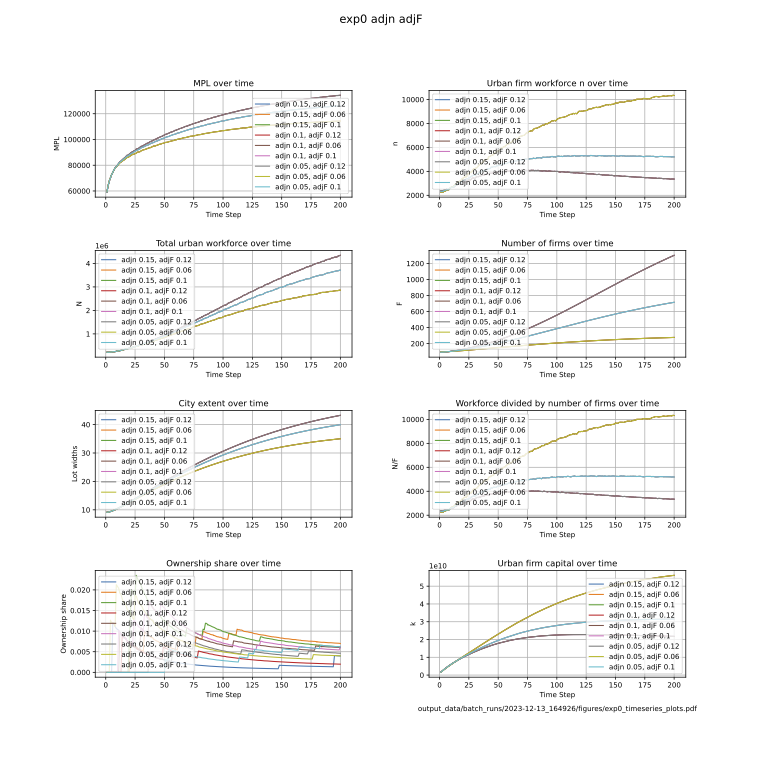
\includegraphics[scale=.55]{fig/Analysis/F-n-adjustment-speed.png}

% Subsistance wage typical 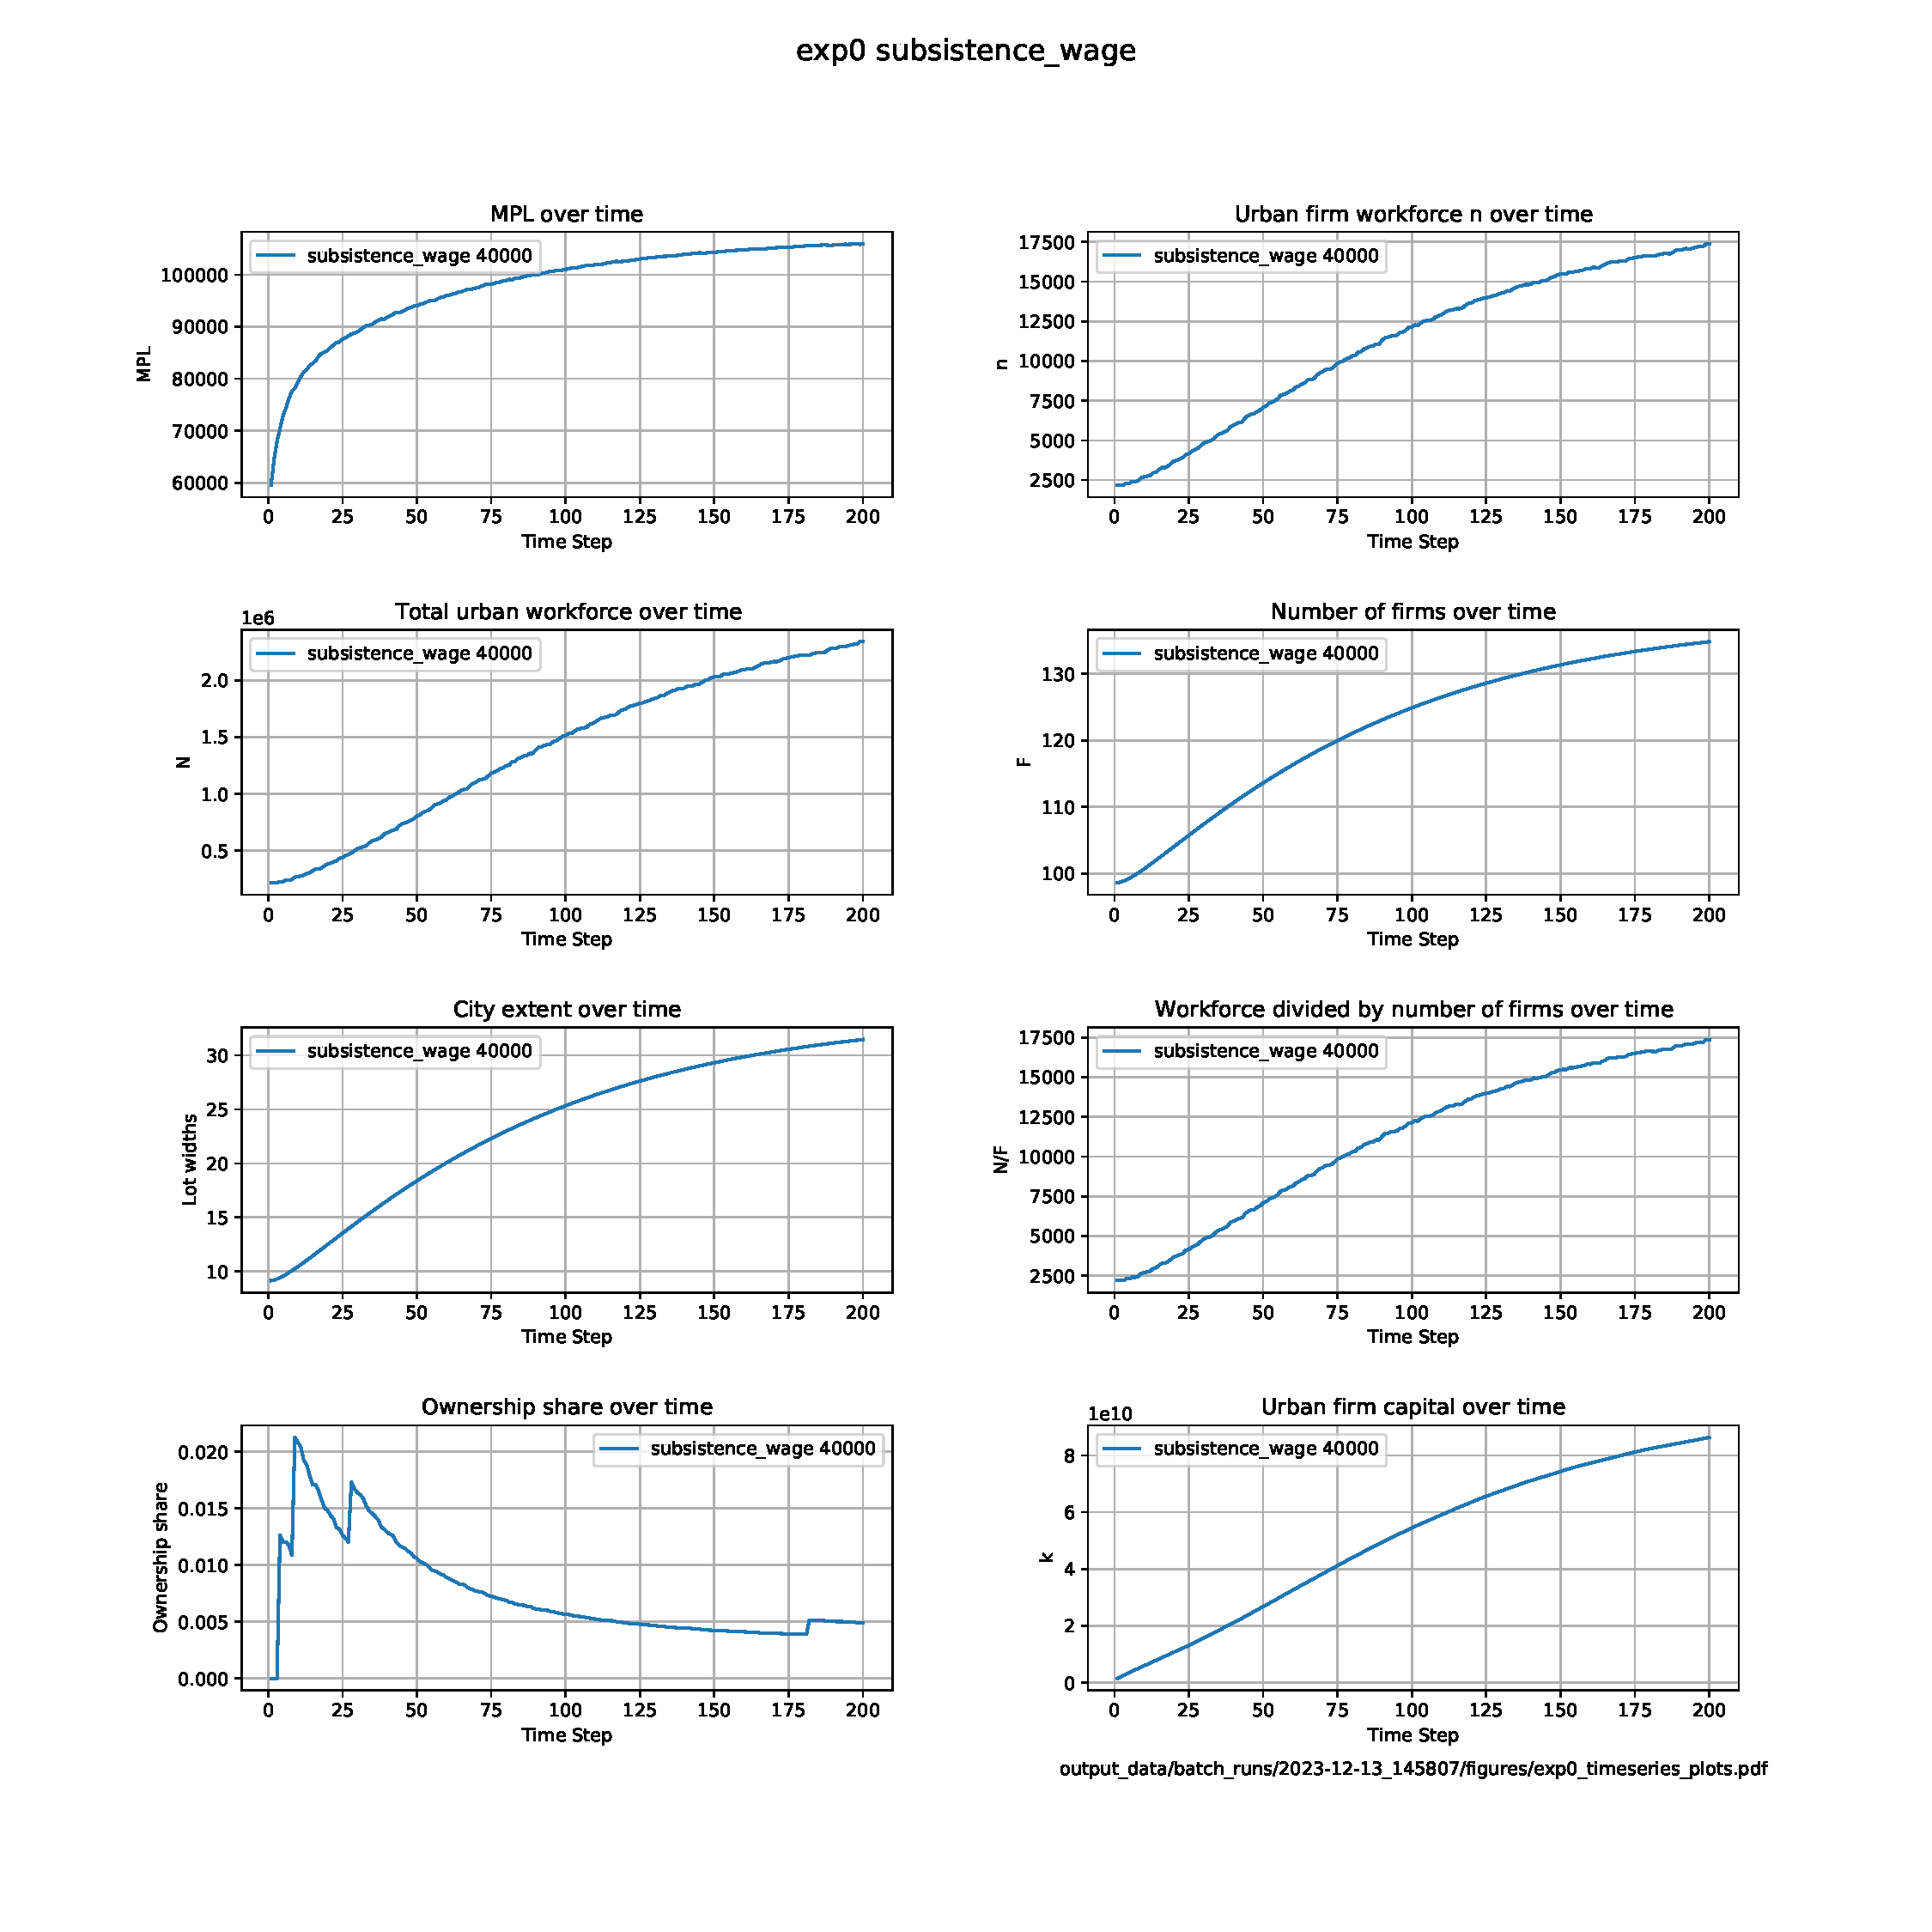
\includegraphics[scale=.55]{fig/Analysis/exp0-timeseries-plots.pdf}


We will want something like this perhaps in an early chapter. this case may not be interesting.
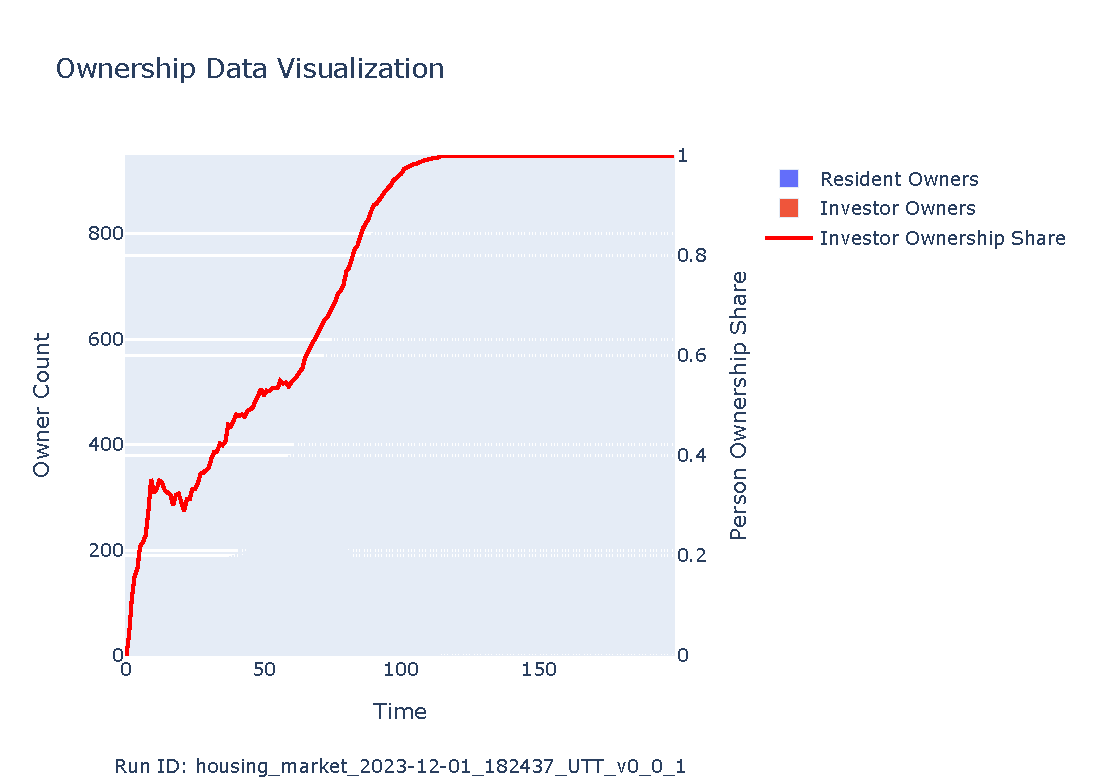
\includegraphics[scale=.95]{fig/Analysis/Ownership_Data_1.pdf}
% \subsection{parameters}
% \begin{verbatim}

% \end{verbatim}
\newpage
% \subsection{parameters}
% \begin{verbatim}

% \end{verbatim}


\newpage %%%%%%%%%%%%%%%%%%%%%%%%%%%%%%%%%%

\subsection{Alpha}
Low levels of capital productivity lead to urban decline. City growth requires a level high enough to overcome decreasing returns in production. 

We do not know why ownership drops suddenly for the very low value of alpha. It happens around the time firm capital peaks

Capital augmenting public expenditures would support growth.
 
% \begin{tabular}{|c|c||c|c||c|c|}
% mpl  & up   & n   & \textbf{down} & N   &  up \\
% F    & up   & E   &  up  &  k & up
% \end{tabular} 

 \hspace*{-2.5cm}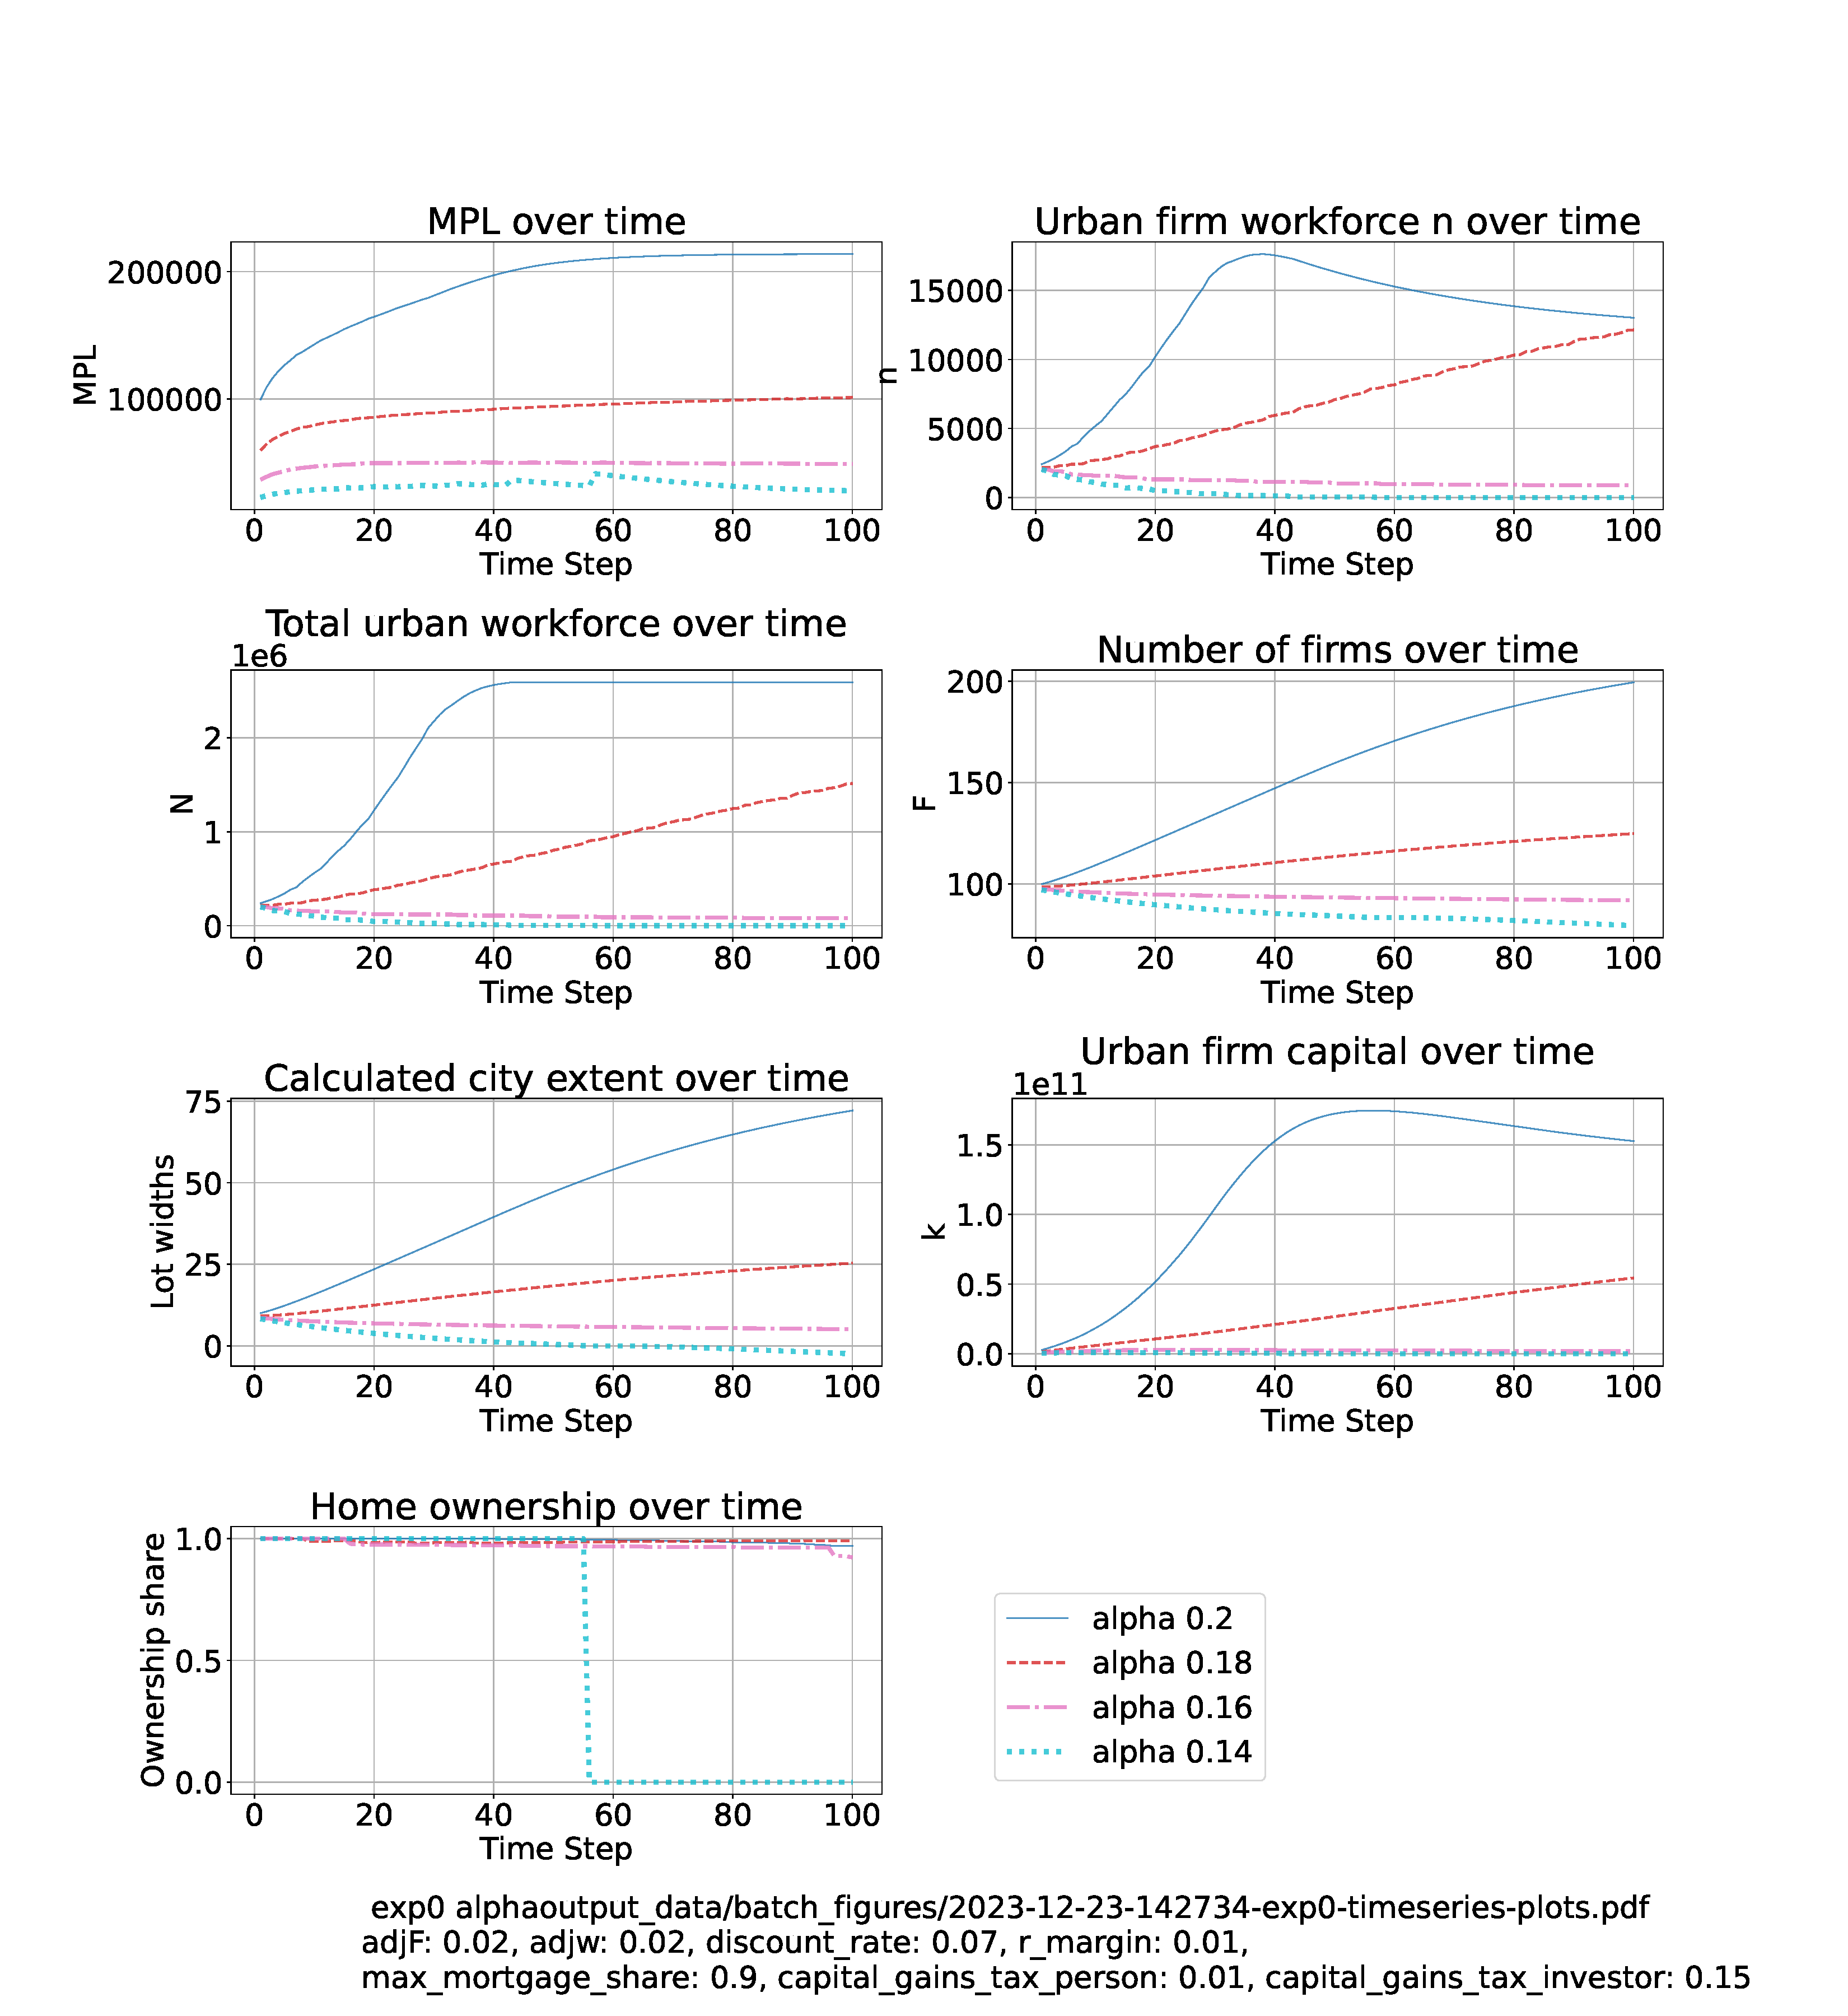
\includegraphics[trim= 1.5cm 3.65cm 2cm 4.0cm, clip, scale=.3]{fig/Analysis/Alpha-4-30.pdf}

\newpage %%%%%%%%%%%%%%%%%%%%%%%%%%%%%%%%%%

\subsection{Transportation cost c}
Transport cost affects the city extent, in turn affecting workforce size and the wealth generated on the city's land. All variables respond as expected. 
 
\begin{tabular}{|c|c||c|c||c|c|}
mpl  & null   & n   & null & N   &  null \\
F    & null   & E   &  null  &  k & null
\end{tabular} 

 \hspace{-2.5cm}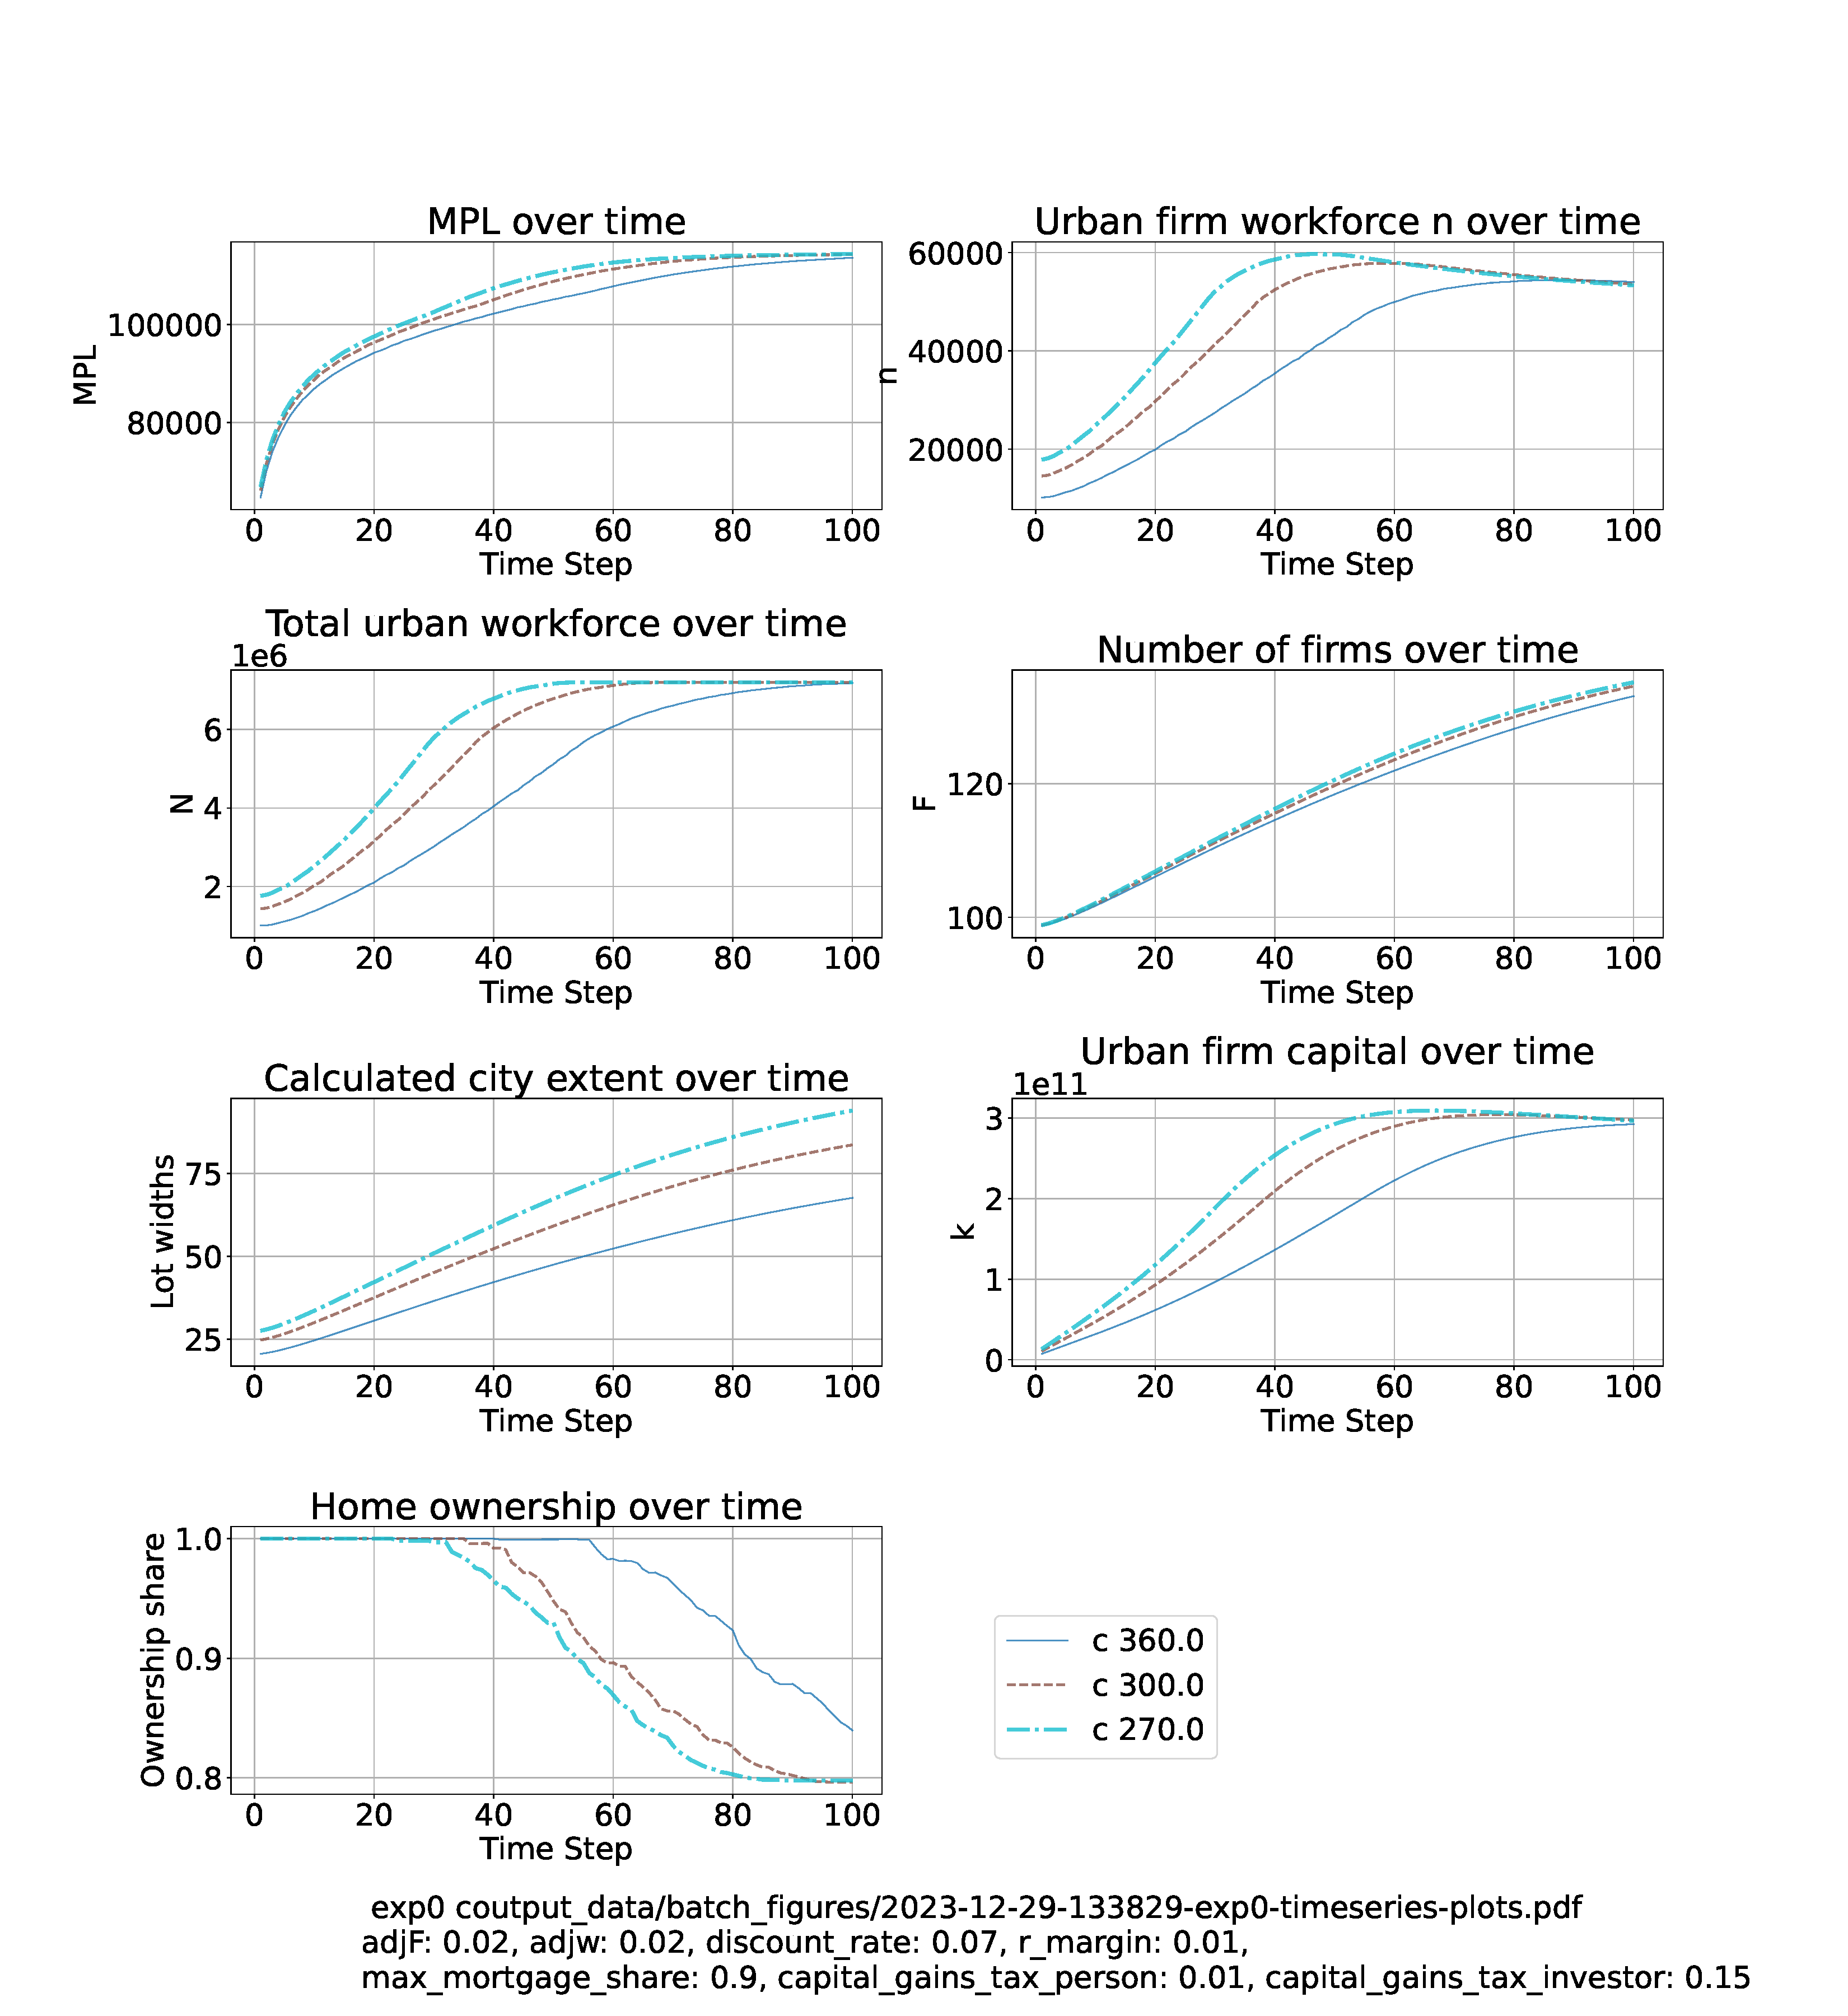
\includegraphics[trim= 1.5cm 3.65cm 2cm 4.0cm, clip, scale=.28]{fig/Analysis/Changing_Transport-cost2.pdf}

Transport cost affects both the total workforce and the total locational rents generated by a city. The response of the workforce is inversely proportional to the square of the transport cost.  

The figure above illustrates 10\% above and below our baseline value.  Reducing transport cost by 10\% increases population and total locational rents 10 \[\frac{1}{0.9 \times 0.9}=1.234568\]
the base value. This calculation assumes that wage and density do not respond as well but that the city extent does adjust.

\[Workforce\propto density * \pi \frac{\omega^2}{c^2}\]
\[Locational\ rents\propto density * \pi \frac{\omega^3}{c^2}\]\

\textbf{These relationships make transport costs the most influential single variable controlled by local authorities.} Transport systems, however, are costly in terms of land use and externalities generated or forgone.

The impact on housing ownership is curious. Home-ownership declines to about 



\newpage %%%%%%%%%%%%%%%%%%%%%%%%%%%%%%%%%%
\section{Housing sector parameters}

\subsection{Capital Gains Taxation}



Capital Gains taxes regulate the amount of future rents that owners capture.  In our model, with two classes of owners, the relative levels of capital gains taxes shift the advantage between owner-occupiers and investors, so we expect variations to affect the ownership share.


Absolute levels of capital gains taxes shift the productivity of the city from the private to the public sector. \textbf{In the current version the tax  revenues are not allocated.  In practice capital gains are a form of income and the revenues from income taxes all  go the the Federal and Provincial governments. They are not fed back into the urban economy. Since they arise form the urban process, policy makers should consider returning them to the Urban system.} 

 The following figure illustrates such a transition over a very small shift in capital gains tax for owners while holding the tax for investors constant at 15\%.

There is no noticeable sensitivity in any base outputs for this parameter. 

Ownership share exhibits a tipping point at a personal capital gains tax rate  near 25\% when the capital gains rate for investors is 15\%  

\vspace{1cm}

% 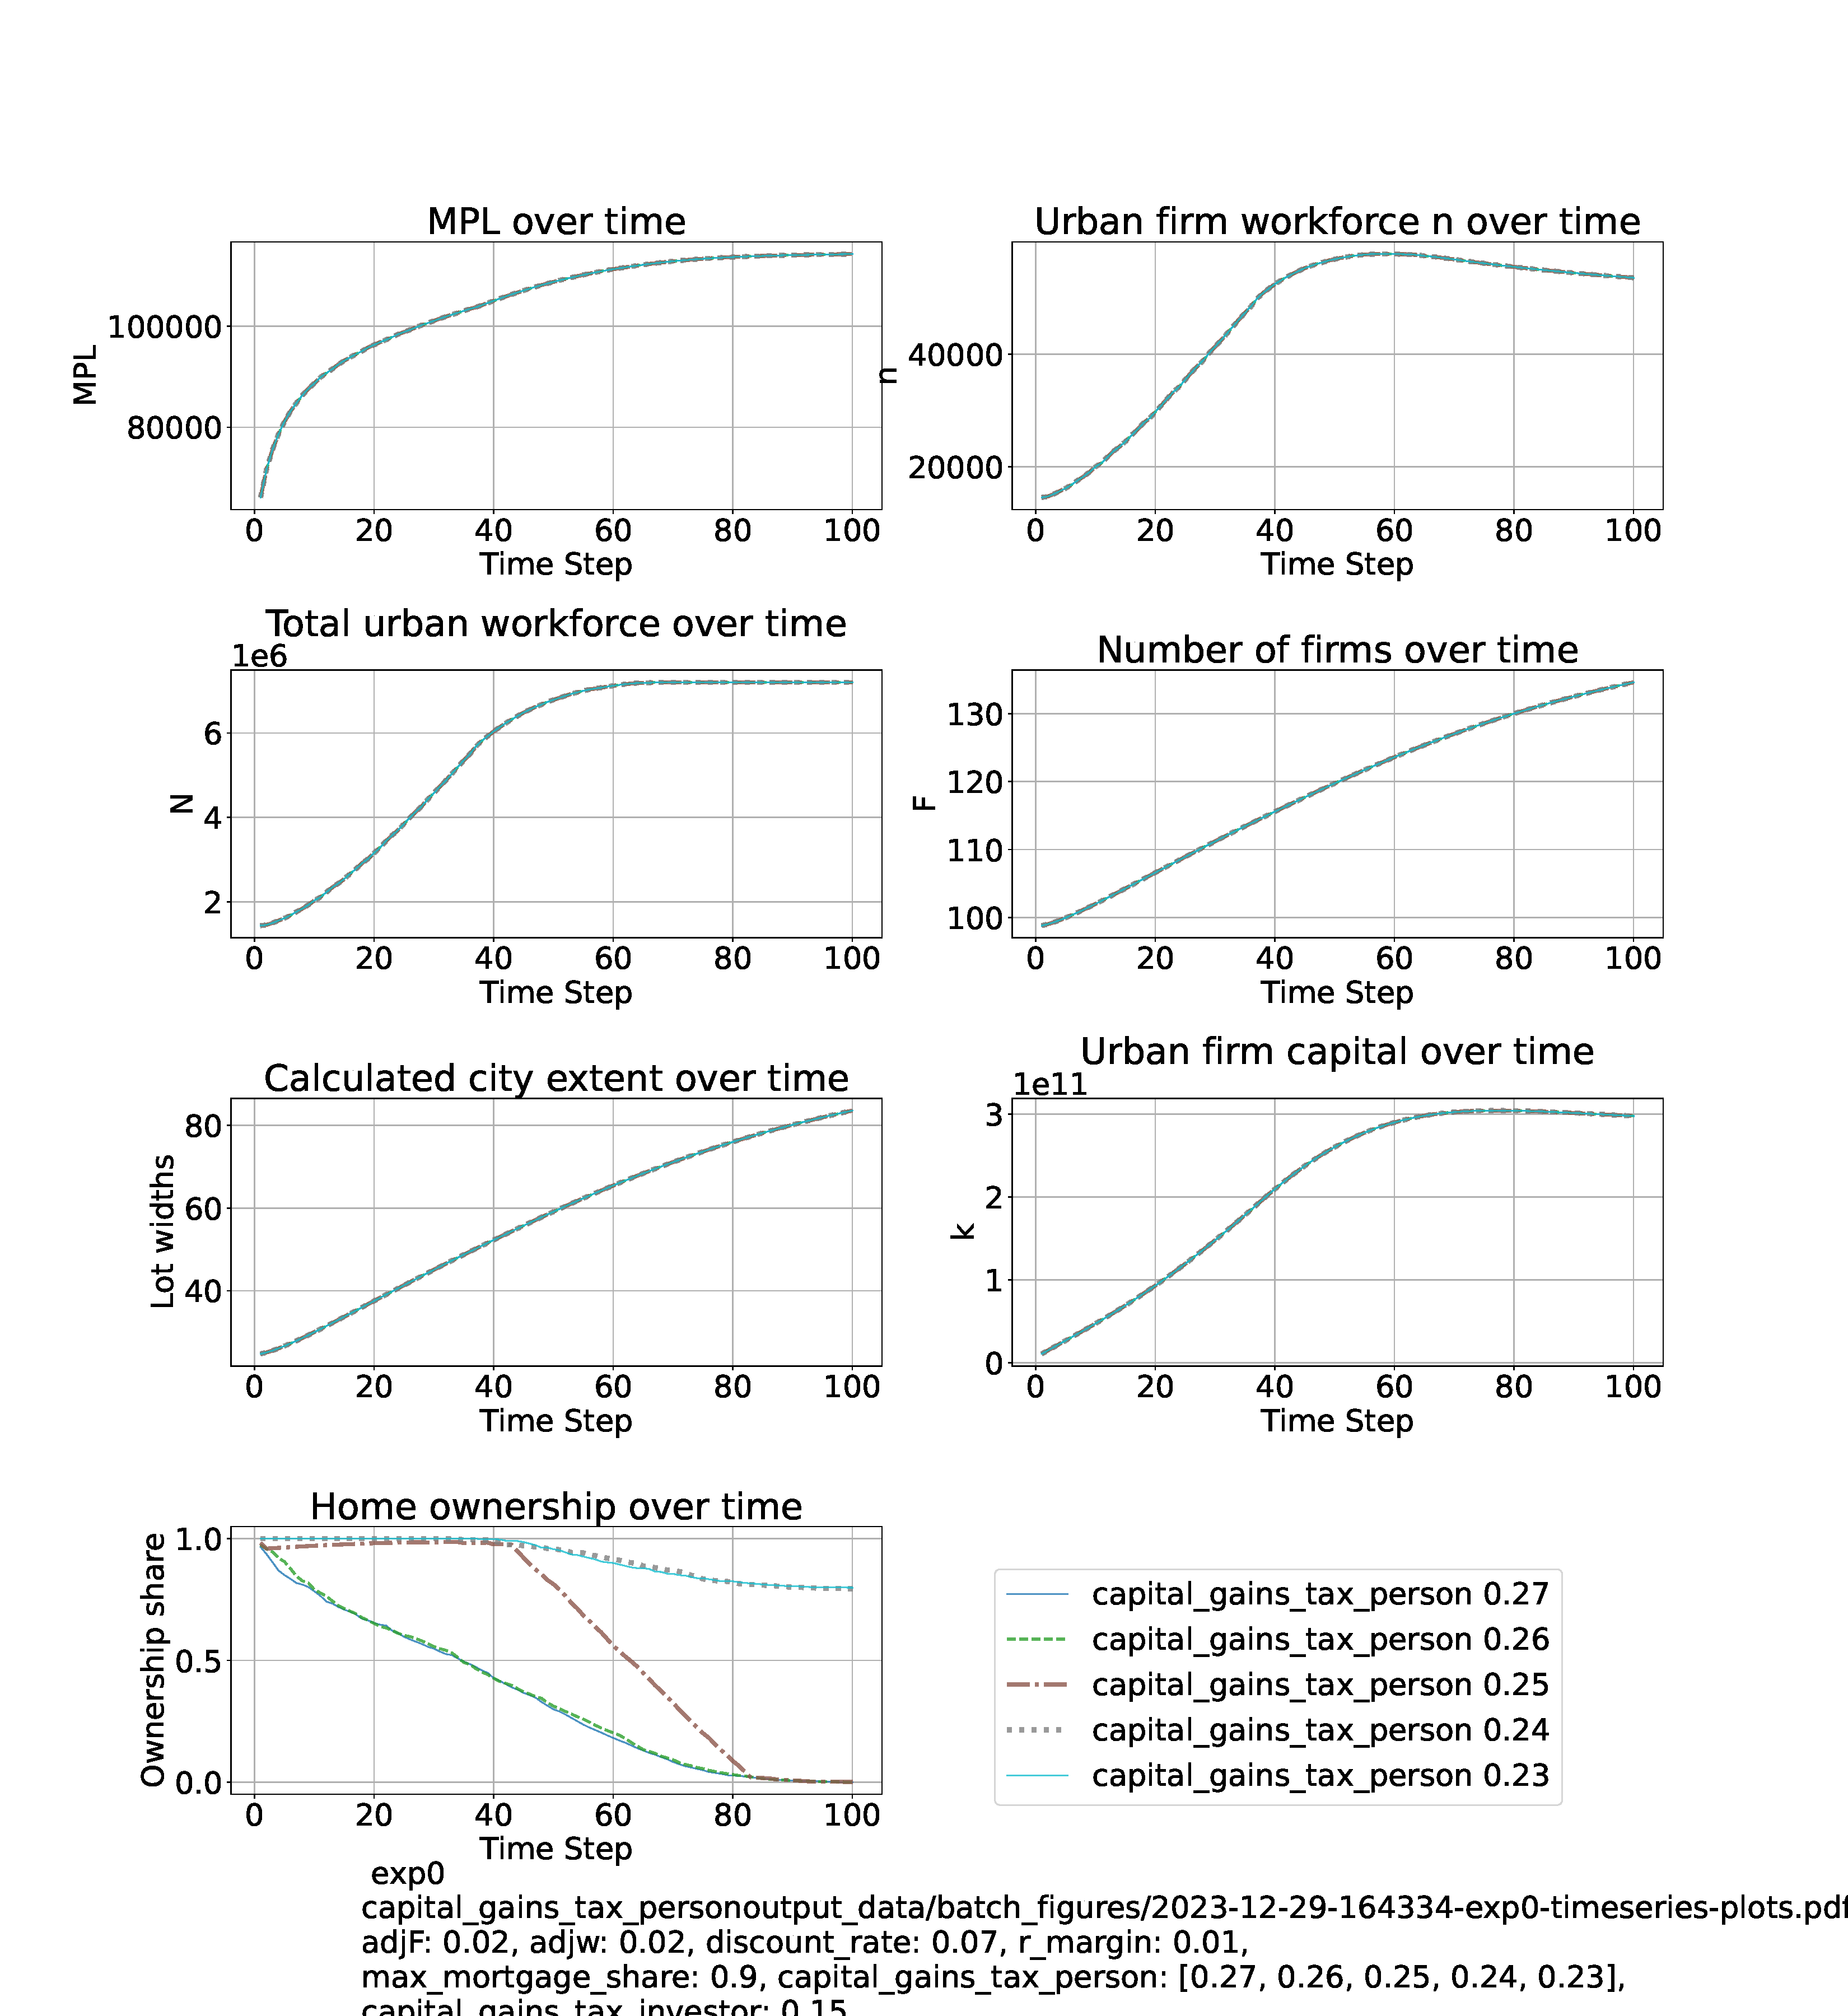
\includegraphics[trim= 1.5cm 3.65cm 2cm 4.0cm, clip, scale=.28]{fig/Analysis/Capital-gains-person-point27-6-5-4-3.pdf}


More precisely, we find that ownership stabilizes at 80\%  capital gains tax rates below 0.245. \textbf{(A gap is 0.1 in favour of households seems to be needed to support home-ownership.)}

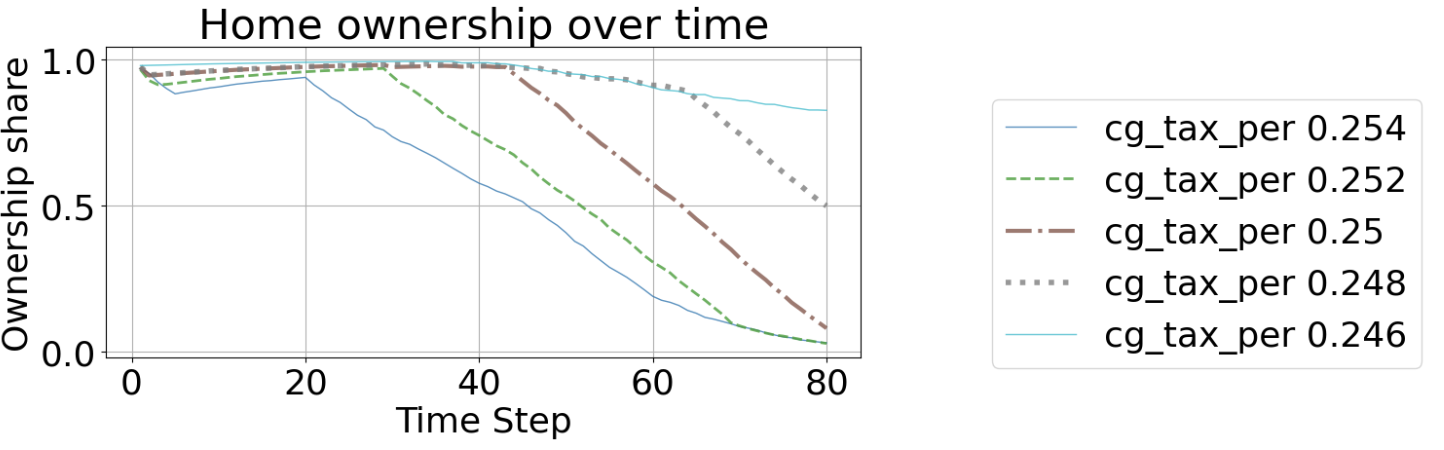
\includegraphics[ scale=.5]{fig/Analysis/Capital-gains-person-point246-254.png}


It should be possible to identify a boundary in the entire capital gains tax space between values of capital gains for investors and occupiers -owners where ownership begins to shift from occupiers to investors.

\vspace{1cm}
WORK IN PROGRESS

When the capital gains rate for \textbf{investors} is varied 

\newpage %%%%%%%%%%%%%%%%%%%%%%%%%%%%%%%%%%


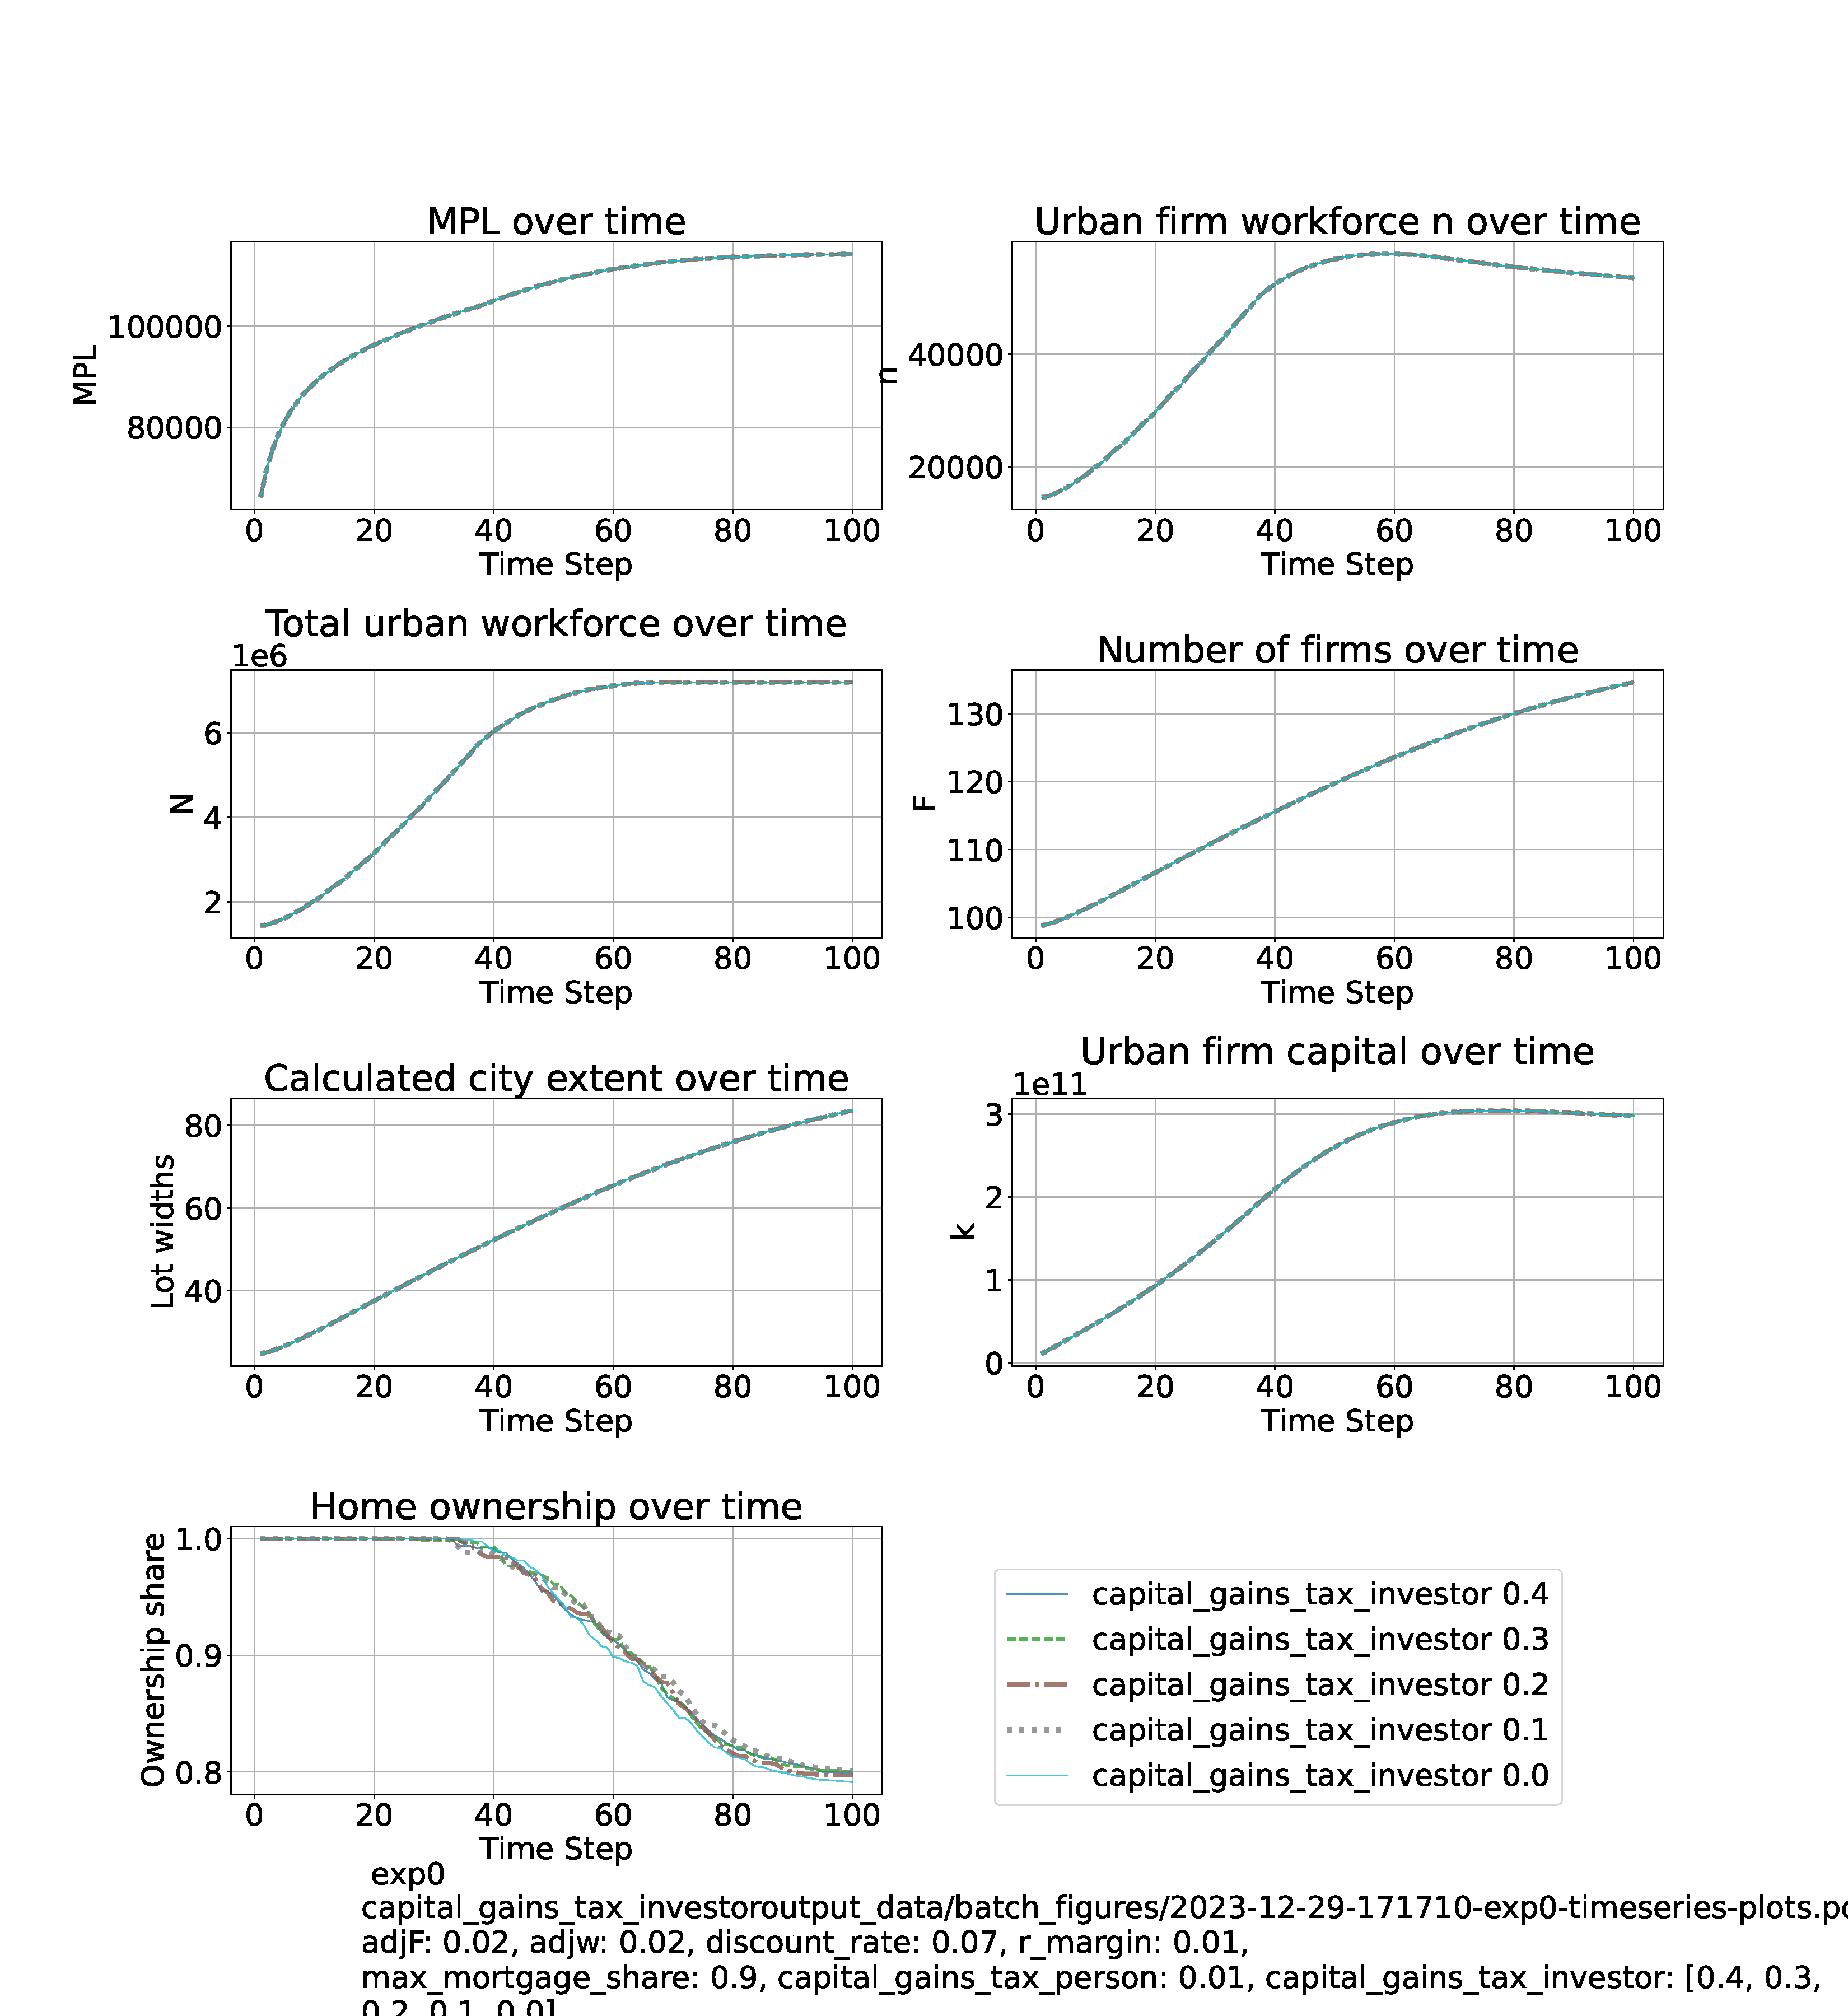
\includegraphics[trim= 1.5cm 3.65cm 2cm 4.0cm, clip, scale=.28]{fig/Analysis/Capital-gains-investor-point-4-3-2-1-0.pdf}



%%%%%%%%%%%%%%%%%%%%%%%%%%%%%%%%%%%%%%%%%%%%%
\newpage
\subsection{Working period}
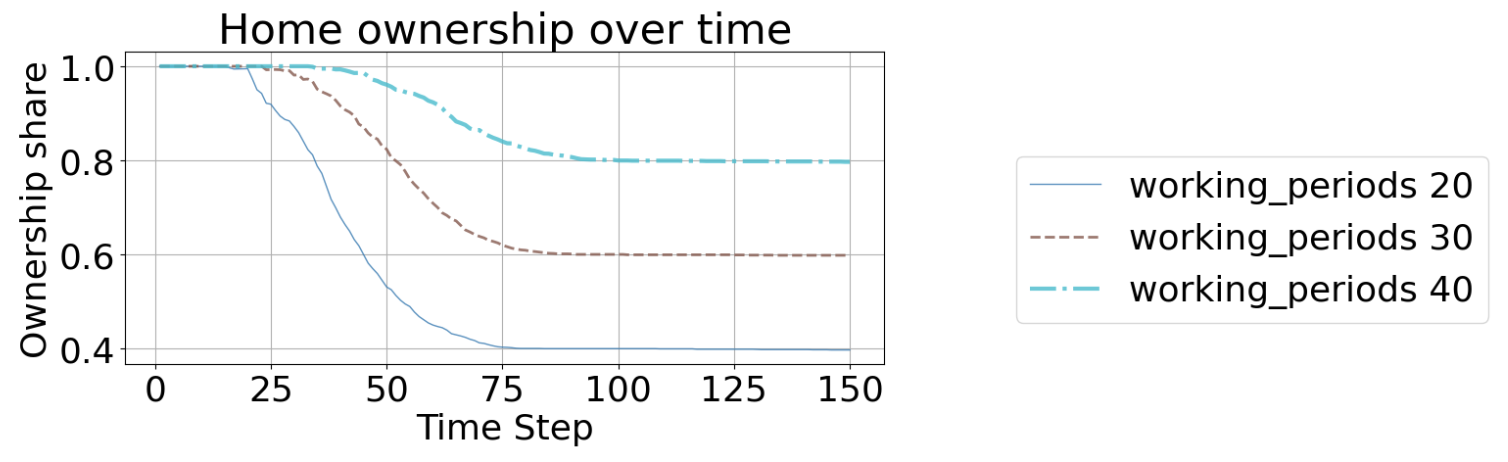
\includegraphics[ scale=.5]{fig/Analysis/Working-period 20-30-40.png}

The longer workers stay in the labour force the higher the fraction of the housing stock that is owner-occupied. this was an unexpected result. 

It is probably because when turnover is increased  institutional investors have m0re chances to get into the market. 

Savings for potential buyers are not obviously affected.

Shorter periods for owners to make capital gains may have an effect.

If the result reflects real processes, it is likely that increased workforce churn reduces owner-occupancy.





\subsection{Maximum Mortgage share}
Contrary to our expectations, the maximum fraction of a come that can be mortgaged appears not to affect  the base economic model and no effect on the pattern of ownership

\subsection{Income share used for mortgage}
This variable also has no effect. Combinations with Maximum Mortgage share have no effect.

%%%%%%%%%%%%%%%%%%%%%%%%%%%%%%%%%%
\newpage
\subsection{Property taxes}

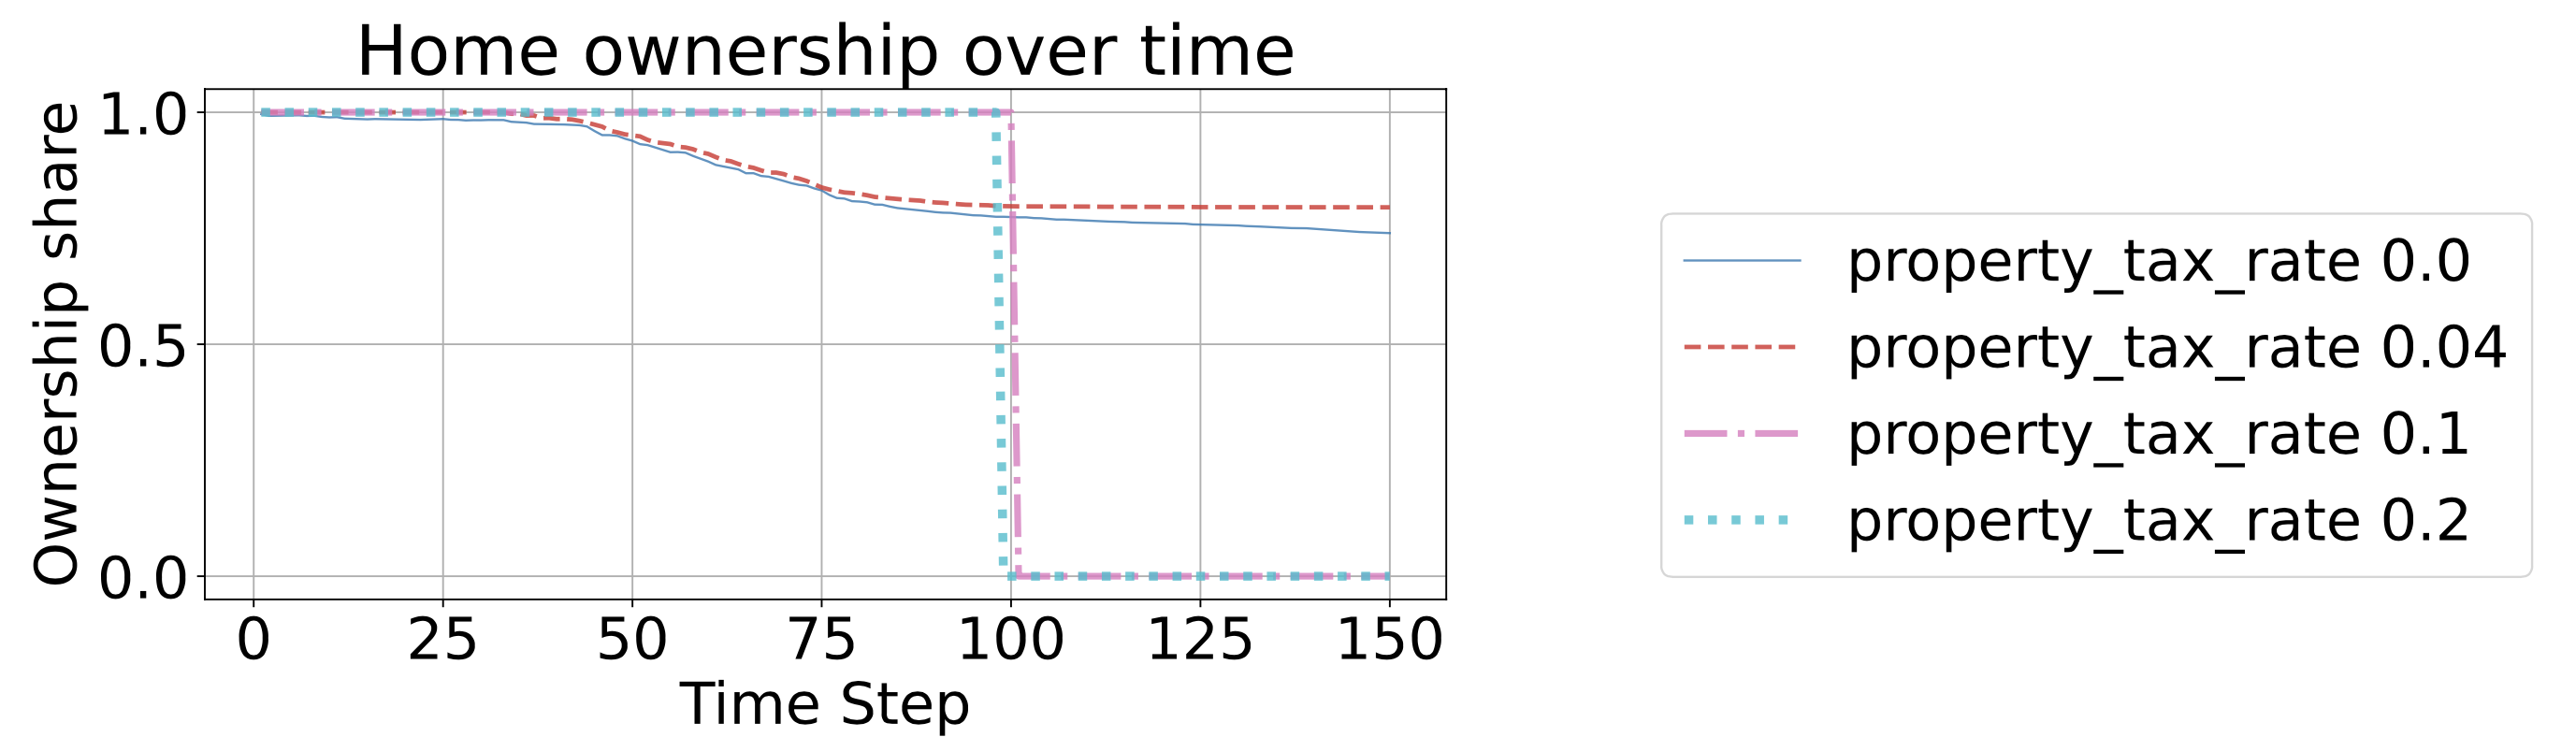
\includegraphics[ scale=.25]{fig/Analysis/Property-tax-point4-2.png}
At a property tax rate of 4.5\% we see a sharp change in the ownership pattern. Above this point owner-occupiers disappear. This seems reasonable, but the time pattern is strange. Why a sharp change at 100 time steps?

4\% approximates the level of actual mill-rates in Ontario.




% %%%%%%%%%%%%%%%%%%%%%%%%%%%%%%%%%%

% \subsection{Working period}

% 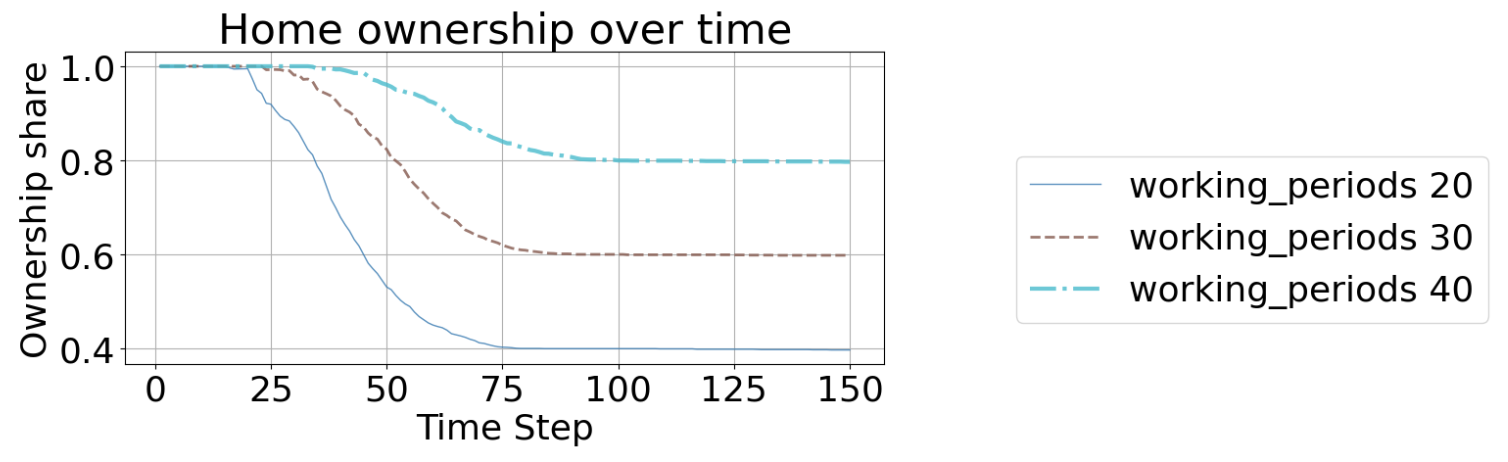
\includegraphics[ scale=.5]{fig/Analysis/Working-period 20-30-40.png}


%%%%%%%%%%%%%%%%%%%%%%%%%%%%%%%%%%
\subsection{12-15 -010050 Change wealth sensitivity two cases 0.1 and 0.05 }
no sensitivity in any output for this parameter base. Ownership share may show  a small effect if we are near a tipping point driven by p-dot

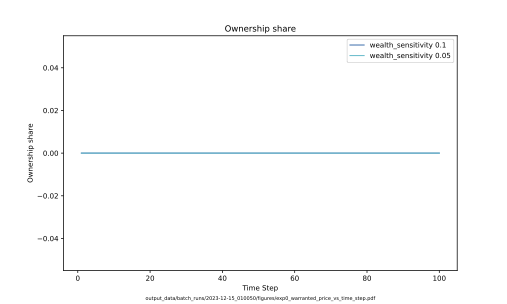
\includegraphics[scale=.45]{fig/Analysis/exp0_warranted_price_vs_time_step.png}


\begin{multicols}{2}
[\textbf{parameters}]
\begin{verbatim}
'adjn': 0.15,
'adjF': 0.02,
'adjw': 0.05, 
'capital_gains_tax_person':   0.0,
'capital_gains_tax_investor': 1,
\end{verbatim}

\end{multicols}
%%%%%%%%%%%%%%%%%%%%%%%%%%%%%%%%%%%%%%%%%%%%%

% %%%%%%%%%%%%%%%%%%%%%%%%%%%%%%%%%%%%%%%%%%%%
%  \subsection{12-17 010050, Varying Capital gains  }
% \begin{tabular}{c|c}
%   mpl  &  \\
%   n   &  \\
%   N   &  \\
%   F   &  \\
%   E   &  \\
%   k   & 
% \end{tabular} 

% \includegraphics[trim= 1.5cm 5cm 2cm 6.5cm, clip, scale=.40]{fig/Analysis/215330-exp0-timeseries-plots.pdf}

% adjF: 0.02, adjw: 0.15, discount_rate: 0.07, r_margin: 0.01, max_mortgage_share: 0.9,  capital_gains_tax_person: [0.5, 0.01], capital_gains_tax_investor: [0.75, 0.5, 0.25

% \includegraphics[scale=.4, trim=2cm  5cm 2cm 4cm, clip]{fig/Analysis/2023-12-17_215330_exp0_timeseries_plots.pdf}

 \end{document}

 \newpage
% \subsection{parameters}
% \begin{verbatim}

% \end{verbatim}

% \subsection{Change  12-15 010050}
\begin{tabular}{c|c}
  mpl  &  \\
  n   &  \\
  N   &  \\
  F   &  \\
  E   &  \\
  k   & 
\end{tabular} 

 \includegraphics[scale=.25]{215330-exp0-timeseries-plots.pdf}
